\documentclass[10pt,a4paper]{article}
\usepackage[
    a4paper,
    top=2.5cm,
    bottom=2.5cm,
    left=2.5cm,
    right=2.0cm,
    bindingoffset=0.5cm,
    headheight=17pt,
    headsep=0.6cm,
    footskip=1.1cm
]{geometry}

\usepackage{afterpage}
\usepackage{diagbox}
\usepackage[UTF8,heading = true]{ctex}
\usepackage{amsmath,amssymb,amsfonts,mathrsfs}
\usepackage{graphicx}
\usepackage{ulem}
\usepackage{pdfpages}
\usepackage{lipsum}
\usepackage{booktabs}
\usepackage{array,tabularx,longtable}
\newcolumntype{Y}{>{\centering\arraybackslash}X}
\usepackage{multirow}
\usepackage{listings}
\usepackage{enumerate}
\usepackage{indentfirst}
\usepackage{tikz}
\usepackage{tikz-qtree,tikz-qtree-compat}
\usetikzlibrary{arrows}
\usepackage{siunitx}
\usepackage{anyfontsize}
\usepackage{fontspec}
\setmainfont{Times New Roman}
\usepackage{xeCJK}
\newcommand{\thesisfontpath}{./}
\newcommand{\songtifakebold}{6.0}
\newcommand{\heitifakebold}{3.5}
\IfFileExists{SimSun.TTC}{}{
    \IfFileExists{latex/SimSun.TTC}{
        \renewcommand{\thesisfontpath}{latex/}
    }{}
}
\IfFileExists{\thesisfontpath SimSun.TTC}{
    \setCJKmainfont[Path=\thesisfontpath,AutoFakeBold=\songtifakebold]{SimSun.TTC}
    \newCJKfontfamily\thesissong[Path=\thesisfontpath,AutoFakeBold=\songtifakebold]{SimSun.TTC}
}{
    \setCJKmainfont[
        UprightFont = * Regular,
        BoldFont = * Bold
    ]{Songti SC}
    \newCJKfontfamily\thesissong[
        UprightFont = * Regular,
        BoldFont = * Bold
    ]{Songti SC}
}
\IfFileExists{\thesisfontpath SimHei.TTF}{
    \setCJKsansfont[Path=\thesisfontpath,AutoFakeBold=\heitifakebold]{SimHei.TTF}
    \newCJKfontfamily\thesishei[Path=\thesisfontpath,AutoFakeBold=\heitifakebold]{SimHei.TTF}
}{
    \setCJKsansfont[
        UprightFont = * W3,
        BoldFont = * W6
    ]{Hiragino Sans GB}
    \newCJKfontfamily\thesishei[
        UprightFont = * W3,
        BoldFont = * W6
    ]{Hiragino Sans GB}
}
\renewcommand{\songti}{\thesissong}
\renewcommand{\heiti}{\thesishei}
\usepackage{setspace}
\usepackage{color}
\usepackage{titletoc}
\usepackage{etoolbox}
\usepackage[comma]{natbib}
\setcitestyle{numbers,square}
\usepackage[explicit]{titlesec}
\titlespacing*{\section}{0pt}{20pt}{20pt}
\titlespacing*{\subsection}{0pt}{10pt}{10pt}
\titlespacing*{\subsubsection}{0pt}{10pt}{10pt}
\usepackage{algorithm,algorithmic}
\usepackage{float}
\usepackage{subfigure}
\usepackage[subfigure]{tocloft}
\usepackage{fancyhdr}
\usepackage{caption}
\usepackage{threeparttable}

\ctexset{
    section={
        name={第,章},
        format=\bfseries\centering\heiti\zihao{-3},
        numberformat=\bfseries\heiti\zihao{-3},
    },
    subsection={
        format=\bfseries\heiti\zihao{4},
        numberformat=\bfseries\heiti\zihao{4}
    },
    subsubsection={
        format=\bfseries\heiti\zihao{-4},
        numberformat=\bfseries\heiti\zihao{-4}
    }
}

\pagestyle{fancy}
\fancypagestyle{thesis}
{
    \fancyhf{}
    \fancyhead[C]{\zihao{5}\songti{\nouppercase{\leftmark}}}
    \fancyfoot[C]{\zihao{5}\songti\thepage}
    \renewcommand{\headrulewidth}{0.5pt}
}
\fancypagestyle{plain}
{
    \fancyhf{}
    \fancyhead[C]{\zihao{5}\songti{\nouppercase{\leftmark}}}
    \fancyfoot[C]{\zihao{5}\songti\thepage}
    \renewcommand{\headrulewidth}{0.5pt}
}
\pagestyle{thesis}

\usepackage[colorlinks,linkcolor=black,citecolor=black,urlcolor=black,filecolor=black,bookmarks=true,bookmarksnumbered=true]{hyperref}

\renewcommand{\cftsecleader}{\cftdotfill{0.6}}
\renewcommand{\cftsubsecleader}{\cftdotfill{0.6}}
\renewcommand{\cftsubsubsecleader}{\cftdotfill{0.6}}
\renewcommand{\cftsecfont}{\zihao{-4}\songti}
\renewcommand{\cftsubsecfont}{\zihao{-4}\songti}
\renewcommand{\cftsubsubsecfont}{\zihao{-4}\songti}
\renewcommand{\cftsecpagefont}{\zihao{-4}\songti}
\renewcommand{\cftsubsecpagefont}{\zihao{-4}\songti}
\renewcommand{\cftsubsubsecpagefont}{\zihao{-4}\songti}
% 目录标题间距与字体：去除 tocloft 默认 50pt 前置空白，居中显示
\setlength{\cftbeforetoctitleskip}{0pt}
\setlength{\cftaftertoctitleskip}{20pt}
\renewcommand{\cfttoctitlefont}{\hfill\zihao{3}\heiti\bfseries}
\renewcommand{\cftaftertoctitle}{\hfill}
\renewcommand{\contentsname}{目\quad 录}

\hypersetup{
    filecolor=black,
    urlcolor=black,
}

\setlength{\parindent}{2em}
\setlength{\parskip}{0pt}
\setlength{\headheight}{17pt}
\setlength{\textfloatsep}{20pt plus 2pt minus 2pt}
\setlength{\intextsep}{20pt plus 2pt minus 2pt}

\DeclareCaptionFont{thesiscaptionfont}{\zihao{5}\songti\setstretch{1}}
\captionsetup{
    labelformat=default,
    labelsep=space,
    justification=centering,
    singlelinecheck=false
}
\captionsetup[figure]{font=thesiscaptionfont,position=bottom,skip=10pt}
\captionsetup[table]{font=thesiscaptionfont,position=top,skip=10pt}

\AtBeginEnvironment{tabular}{\zihao{5}\songti\renewcommand{\arraystretch}{1.6}}
\AtBeginEnvironment{tabularx}{\zihao{5}\songti\renewcommand{\arraystretch}{1.6}}
\AtBeginEnvironment{longtable}{\zihao{5}\songti\renewcommand{\arraystretch}{1.6}}

\numberwithin{equation}{section}
\numberwithin{table}{section}
\numberwithin{figure}{section}
\renewcommand{\theequation}{\thesection-\arabic{equation}}
\renewcommand{\figurename}{图}
\renewcommand{\tablename}{表}
\renewcommand{\sectionmark}[1]{\markboth{第\thesection 章\quad #1}{第\thesection 章\quad #1}}
\renewcommand{\subsectionmark}[1]{}
\newcommand{\thesisbodyfont}{\fontsize{12pt}{20pt}\selectfont\songti}
\newcommand{\thesisenglishfont}{\fontsize{12pt}{20pt}\selectfont}
\newcommand{\frontmattergeometry}{%
    \newgeometry{
        top=2.5cm,
        bottom=2.5cm,
        left=2.5cm,
        right=2.0cm,
        bindingoffset=0.5cm,
        headheight=17pt,
        headsep=0.6cm,
        footskip=1.1cm
    }%
}
\newcommand{\mainmattergeometry}{%
    \newgeometry{
        top=2.5cm,
        bottom=2.5cm,
        left=2.5cm,
        right=2.0cm,
        bindingoffset=0.5cm,
        headheight=17pt,
        headsep=0.9cm,
        footskip=1.4cm
    }%
}

\graphicspath{{pics/}}
\newcommand{\placeholderfigure}[2]{%
    \begin{figure}[htbp]
        \centering
        \setlength{\fboxsep}{0pt}%
        \fbox{%
            \parbox[c][5.2cm][c]{0.82\textwidth}{%
                \centering
                \zihao{5}\songti 图像占位\\[6pt]
                \zihao{-4}\songti 后续补充正式图片%
            }%
        }
        \caption{#1}
        \label{#2}
    \end{figure}
}

\begin{document}
    \bibliographystyle{plainnat}
    \includepdf{cover.pdf}
    \frontmattergeometry
    \pagenumbering{Roman}
    \setcounter{page}{1}
    \renewcommand{\thesubfigure}{\empty}

    \markboth{摘要}{摘要}
    \phantomsection
    \addcontentsline{toc}{section}{摘要}

    \vspace*{0pt}
    \centerline{\zihao{3}\heiti\bfseries 摘\quad 要}
    \vspace*{16pt}

    {\thesisbodyfont
    随着“双碳”目标的推进与电动汽车规模化发展，充电负荷的时空不确定性对配电网安全运行构成挑战。本文围绕充电负荷时空建模与配电网承载力概率评估展开研究。首先，构建基于出行链的多日连续仿真模型，刻画日内多次出行、驻留、充电全过程，生成母线级时序负荷矩阵。其次，提出硬约束与软指标双层评估体系，以蒙特卡洛概率评估为核心，辅以确定性和灵敏度方法，通过自适应二分搜索求解最大可接纳电动汽车规模 $N^*$。最后，设计融合五因子动态评分的充电导航策略，量化空间引导对承载力的提升效果。以改进 IEEE 33 节点系统为算例，仿真表明：出行链模型下无序充电承载力为 85 辆，导航策略提升至 101 辆，增幅约 19\%；三种方法所得承载力呈确定性（7 辆）$<$灵敏度（24 辆）$<$蒙特卡洛（85 辆）的递增关系；电压约束为系统唯一瓶颈，母线 17 为最薄弱节点。
    \par}

    \bigskip
    {\thesisbodyfont\noindent\textbf{关键词：} 电动汽车；出行链；配电网承载力；蒙特卡洛模拟；充电导航\par}

    \newpage
    \phantomsection
    \addcontentsline{toc}{section}{Abstract}
    \markboth{Abstract}{Abstract}
    \vspace*{0pt}
    \centerline{\zihao{3}\bfseries Abstract}
    \vspace*{16pt}

    {\thesisenglishfont
    With China's carbon peak and carbon neutrality goals driving rapid electric vehicle (EV) adoption, the pronounced spatio-temporal uncertainty of charging loads poses significant challenges to distribution network operation. This paper presents a systematic study on spatio-temporal modeling of EV charging loads and probabilistic hosting capacity assessment of distribution networks. First, a trip-chain-based multi-day continuous simulation model is developed to capture the complete daily cycle of travel, parking, and charging behaviors, thereby generating bus-level time-series charging load matrices. Second, a dual-layer assessment framework combining hard constraints and soft indicators is proposed. Monte Carlo probabilistic evaluation serves as the core method, supplemented by deterministic assessment and voltage sensitivity analysis, while an adaptive binary search algorithm is employed to determine the maximum admissible EV count $N^*$. Third, a charging navigation strategy incorporating a five-factor dynamic scoring mechanism is designed to guide spatial redistribution of charging loads and quantify the resulting hosting capacity improvement. Simulation results on the modified IEEE 33-bus system demonstrate that the hosting capacity under uncontrolled charging with the trip-chain model is 85 EVs, which the navigation strategy increases to 101 EVs, representing a 19\% improvement. The three assessment methods yield hosting capacities of 7, 24, and 85 EVs, respectively. Voltage constraint is identified as the sole binding factor, with Bus 17 as the weakest node.
    \par}

    \bigskip
    {\thesisenglishfont\noindent\textbf{Key words：} electric vehicle; trip chain; distribution network hosting capacity; Monte Carlo simulation; charging navigation\par}

    \newpage
    \markboth{目录}{目录}
    \setcounter{secnumdepth}{3}
    \setcounter{tocdepth}{2}

    \begin{spacing}{1.7}
        \tableofcontents
    \end{spacing}
    \vspace*{16pt}

    \newpage
    \mainmattergeometry
    \pagestyle{thesis}
    \pagenumbering{arabic}
    \setcounter{page}{1}
    \thesisbodyfont

    \section{绪论}
    \markboth{\text{第}\thesection\text{章} \quad 绪论}{\text{第}\thesection\text{章} \quad 绪论}

    \subsection{研究背景与意义}

    面对全球气候变化的严峻挑战，我国明确提出 2030 年前实现碳达峰、2060 年前实现碳中和的“双碳”战略目标。交通运输行业作为碳排放的重点领域，其电气化转型是实现减排目标的重要抓手。近年来，在产业政策扶持与技术进步的双重驱动下，我国电动汽车产业发展迅速。据统计，2021 年我国新能源汽车销量突破 350 万辆[1]，随后连续数年保持高速增长，电动汽车保有量已居全球首位。电动汽车的规模化推广推动能源消费结构从“油”向“电”转移，在降低交通碳排放的同时，也对配电侧基础设施的容量与运行安全提出了新的挑战。

    电动汽车充电负荷的本质特征在于其时空分布的强不确定性。在时间维度上，充电需求的产生取决于用户的日常出行规律，出发时刻、行驶距离、驻留时长等行为参数均服从特定的概率分布，不同用户之间存在显著差异[2]。在空间维度上，车辆随出行在居住区、工作区、商业区等城市功能区之间迁移，充电需求随之在不同区域的充电设施间转移[3]。这种“出行、交通、充电”的耦合特性使得充电负荷在时间和空间上的演化规律远较传统居民或工业负荷复杂[4]。

    当大量电动汽车在缺乏协调的情况下接入配电网时，其充电行为可能引发多重运行问题。Powell 等[5]的研究表明，在电动汽车高渗透率情景下，电网峰值净需求可增加 25\%，完全电气化极端情景下增幅可达 50\%。具体而言，充电负荷与居民晚高峰负荷在时间上高度重合，形成“峰上加峰”效应，致使配电变压器与馈线面临过载风险；大量有功负荷注入导致线路压降增大，配电网末端节点电压跌落至安全限值以下；线路电流的增大同时引起 $I^2R$ 损耗显著上升，降低网络运行经济性[6]。这些问题在充电设施密集、电动汽车渗透率较高的区域尤为突出。

    在此背景下，配电网承载力（Hosting Capacity, HC）概念被引入以量化电网对新型负荷的接纳能力。承载力定义为：在满足电压质量、热稳定性及设备容量等运行约束，且无需进行大规模网络升级的条件下，配电网可接纳的电动汽车最大规模或最大等效充电功率[6]。Fatima 等[6]的综述指出，已有文献中约 57\% 将电压越限作为承载力的主要约束因素，约 41\% 考虑了变压器过载约束，约 36\% 采用了线路热容量约束。承载力评估已从传统的“单节点、单时刻”静态校核，发展为“多时段、多场景、多指标”的综合评估，尤其需要计及充电负荷的时空分布特性与随机性。

    \begin{figure}[htbp]
        \centering
        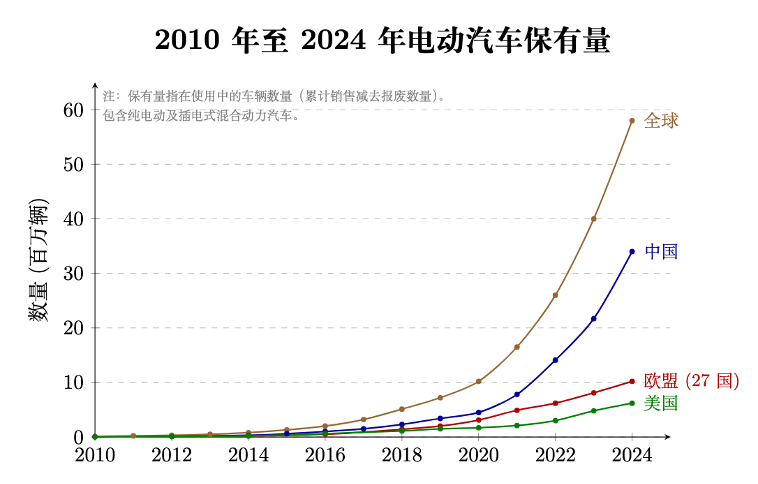
\includegraphics[width=0.82\textwidth]{1-1.png}
        \caption{我国新能源汽车保有量变化趋势}
        \label{fig:ev_population}
    \end{figure}

    本课题的研究具有理论与工程双重意义。在理论层面，本研究将承载力评估的对象从传统分布式电源拓展至电动汽车充电负荷，重点刻画负荷的时空迁移与随机特征，推动交通、电力耦合建模方法的深化融合。在工程应用层面，承载力评估结果与薄弱环节定位可直接指导配电网的规划决策，包括变压器扩容、线路改造等工程措施的优先排序，以及充电站选址与容量配置的优化。此外，量化空间调度策略对承载力的提升效果，可为运营商制定充电引导方案提供定量依据，在不增加物理投资的前提下提升配电网的电动汽车接纳能力。

    \subsection{国内外研究现状}

    \subsubsection{电动汽车充电负荷时空建模}

    电动汽车充电负荷的准确建模是承载力评估的前提与基础。陈丽丹等[2]在综述中系统梳理了充电负荷预测方法，将其分为统计概率法、出行链法、多智能体法、数据驱动法等类别，指出充电负荷的时空特性受电池参数、出行行为、交通路况及充电设施布局等多因素耦合影响。围绕时空建模问题，国内外学者从不同角度进行了深入研究。

    \noindent\textbf{（1）统计概率法}

    早期研究多采用基于统计概率分布的建模方法。田立亭等[7]基于美国全国家庭出行调查（NHTS）数据，以充电起始时刻和日行驶里程为核心随机变量建立充电功率需求的概率模型，其中起始充电时间服从均值为 17.6 h、标准差为 3.4 h 的正态分布，日行驶里程服从对数正态分布。该方法假设车辆一日一充，通过蒙特卡洛抽样生成聚合充电负荷曲线。罗卓伟等[8]进一步按私家车、出租车、公务车、公交车四种类型分别建立充电负荷计算模型，考虑了不同车型在充电时段、充电频次和 SOC 初始分布上的差异。统计概率法原理清晰、实现简便，但由于假设一日仅充电一次且未刻画日内多次出行的行为细节，难以捕捉充电负荷在时间和空间上的精细分布特征。

    \noindent\textbf{（2）出行链法}

    为弥补统计法在行为刻画上的不足，出行链方法逐步成为主流建模范式。出行链将电动汽车日内活动描述为“出行、驻留”交替的完整序列，如“家 $\rightarrow$ 通勤 $\rightarrow$ 工作 $\rightarrow$ 购物 $\rightarrow$ 家”，每一环节的随机变量通过概率分布独立刻画，同时考虑环节间的时间耦合约束。

    陈丽丹等[9]较早地提出了基于出行链的充电负荷预测模型，将日内出行活动划分为家（H）、工作（W）、购物餐饮（SE）、社交娱乐（SR）和其他事务（O）五种类型，采用三参数 Weibull 函数拟合各行程结束时刻的分布，并引入行程约束系数处理链内各段的时间耦合关系。该模型进一步考虑了温度与交通状况对行驶能耗的影响，通过蒙特卡洛模拟获取聚合充电负荷的时空分布。在此基础上，李含玉等[10]将路网模型融入出行链仿真框架，引入基于 Logit 函数的路段阻抗模型和 Dijkstra 最短路径算法，以 1 分钟时间步长模拟车辆在路网中的行驶过程，并建立了充电条件判断的完整流程，同时评估了 V2G 响应潜力。Wang 等[11]采用朴素贝叶斯模型刻画出行行为的随机特征，生成时空耦合的日内行程序列，并对比了仅家庭充电、机会充电和混合充电三种模式对负荷曲线的影响差异。出行链方法的核心优势在于能够在统一框架下刻画日内多次出行的时空分散性，生成的充电负荷在峰值时段、空间分布等方面更为贴近实际。

    \noindent\textbf{（3）车-路-网耦合建模}

    随着研究的深入，学者们开始将交通网络拓扑与配电网络结构进行耦合建模，以实现充电负荷在空间维度上的精确定位。邵尹池等[4]提出了“车-路-网”模式下的充电负荷时空预测方法，在交通网络侧构建了速度、流量模型和交叉口阻抗模型，采用 Floyd 算法实现路径优化，通过蒙特卡洛模拟获取各路网节点的充电需求，再经由路网节点与配电网母线的耦合映射关系将其转化为母线级时序负荷矩阵，在 IEEE 33 节点配电系统上分析了不同场景下充电负荷对节点电压的影响。穆云飞等[12]在此基础上提出了“人-车-桩-路-网”深度耦合的协同规划与运行优化框架，进一步将人的出行行为决策、充电桩布局和电网运行约束纳入统一模型。该类方法能够实现充电负荷的空间精确定位，但也面临交通数据获取难度大、计算开销高等问题。

    \noindent\textbf{（4）数据驱动法}

    近年来，随着充电交易数据和车辆轨迹数据的积累，基于深度学习的数据驱动方法亦得到广泛关注。长短期记忆网络（LSTM）、门控循环单元（GRU）以及时空图卷积网络（ST-GCN）等模型被用于区域充电负荷预测，在捕捉时序模式和空间相关性方面表现出较高精度。然而，此类方法的可解释性不足且对训练数据的质量与规模存在较强依赖，在规划层面的适用性有待验证[2]。

    上述四类方法各有侧重与适用场景，表 \ref{tab:model_compare} 对其进行了系统对比。

    \begin{table}[htbp]
        \centering
        \caption{电动汽车充电负荷建模方法对比}
        \label{tab:model_compare}
        \zihao{5}
        \setlength{\tabcolsep}{4pt}
        \renewcommand{\arraystretch}{1.35}
        \begin{tabularx}{\textwidth}{>{\centering\arraybackslash}p{1.8cm} >{\centering\arraybackslash}p{2.6cm} >{\raggedright\arraybackslash}X >{\raggedright\arraybackslash}X >{\raggedright\arraybackslash}X}
            \toprule
            方法类别 & 代表文献 & 核心思路 & 优势 & 局限 \\
            \midrule
            统计概率法 & 田立亭等[7]、罗卓伟等[8] & 基于充电起始时间与日行驶里程的概率分布，蒙特卡洛抽样生成聚合负荷 & 原理清晰，实现简便，参数可直接由调查数据标定 & 假设一日一充，未刻画日内多次出行的时空分散特征 \\
            出行链法 & 陈丽丹等[9]、李含玉等[10]、Wang 等[11] & 构建日内“出行、驻留”完整序列，各环节参数服从概率分布，仿真单车行为后聚合 & 刻画日内多次出行和充电的行为细节，时空特征更为精细 & 模型参数较多，校准依赖出行调查数据 \\
            车-路-网耦合法 & 邵尹池等[4]、穆云飞等[12] & 在交通网络中进行路径分配与充电需求模拟，通过耦合映射投射至配电网节点 & 实现充电负荷的空间精确定位，可反映交通状态对充电的反馈 & 需要处理大规模交通数据，计算开销较高 \\
            数据驱动法 & LSTM、ST-GCN 等 & 利用历史充电数据训练深度学习模型，直接预测区域充电负荷时序 & 预测精度较高，无需显式物理建模 & 可解释性不足，对数据质量与规模依赖性强 \\
            \bottomrule
        \end{tabularx}
    \end{table}

    \subsubsection{配电网承载力评估方法}

    配电网电动汽车承载力评估旨在确定：在满足电压质量、热稳定性等运行约束的前提下，系统可接纳的最大电动汽车规模或最大充电负荷水平。Fatima 等[6]在综述中系统梳理了承载力的量化与提升方法，指出承载力结果并非电动汽车接入的硬性上限，而是反映各项性能指标在不同渗透率水平下的表现特征。现有研究报告的承载力数值差异较大，城市配电网为 4.7\%$\sim$80\%，郊区为 10\%$\sim$40\%，农村为 10\%$\sim$56\%，具体取值取决于网络结构、充电模式和约束设定等因素。

    \noindent\textbf{（1）确定性评估方法}

    确定性方法以代表性场景或最不利工况为输入，通过逐步增加电动汽车接入规模并进行多时段潮流计算，确定约束首次被违反时对应的最大接入量。陈卫等[13]提出了一套包含电压合格率、线路安全系数、短时负载率、网损率等七项指标的评估体系，采用模糊理论与层次分析法进行综合评分，并结合蚁群算法进行网络重构优化，以 IEEE 33 节点系统为算例验证了方法的有效性。确定性方法计算效率高且结果直观，但由于采用最不利场景假设，所得承载力往往偏于保守，可能导致电网资产利用率偏低。

    \noindent\textbf{（2）概率评估方法}

    为合理处理充电负荷的随机性，概率评估方法应运而生。其核心思想为：通过蒙特卡洛模拟生成大量随机场景，统计给定接入规模下约束被违反的概率，当该违规概率不超过预设的风险容忍度时，对应的接入规模即为概率承载力。郭毅等[14]针对居民区配电网提出了统计评估方法，基于蒙特卡洛模拟结合区域划分进行分层负荷分配，以电压偏差和网损为指标评估电动汽车接纳能力。侯佳欣[15]从时空转移的角度建立了完整的承载力评估框架，以出行链生成充电负荷、潮流计算校验约束、蒙特卡洛统计风险概率为技术路线，采用二分搜索算法求解最大安全接入规模。概率方法通过容许一定的风险概率来释放额外容量，相比确定性方法能够更为合理地评估电网的实际接纳能力。

    \noindent\textbf{（3）鲁棒与分布鲁棒方法}

    当充电负荷的精确概率分布难以获取时，鲁棒优化和分布鲁棒优化（DRO）方法提供了另一类解决思路。Zhao 等[16]提出了电动汽车“可充电区域”（Chargeable Region）概念，将承载力最大化建模为两阶段鲁棒优化问题，在第一阶段优化可充电区域与电网决策变量，在第二阶段校验最恶劣场景下的可行性。黄梦旗等[17]进一步从充电站选择角度建立了电动汽车空间可调度模型，构建了基于 Wasserstein 距离模糊集的两阶段分布鲁棒承载力计算模型，采用列与约束生成算法求解，分析了空间可调度性与设备配置对配电网承载能力的影响。DRO 方法在概率信息有限的条件下兼顾了准确性与鲁棒性，但模型的计算复杂度较高。

    Xi 等[18]将承载力评估的关注点归纳为电能质量（电压偏差、谐波）、运行可靠性（线路负载率、变压器负载率）和运行经济性（网损率）三个维度，指出随着电动汽车接入规模增大，线路载流能力和负荷峰谷特性逐渐成为制约承载力的主要因素。

    综观已有研究，承载力评估方法经历了从确定性到概率性再到鲁棒性的发展历程，评估精度与计算复杂度之间的权衡始终是方法选择的核心考量。同一系统采用不同方法所得承载力可能存在数量级差异，如何系统对比并揭示各方法的适用边界仍是值得深入探讨的问题。

    \subsubsection{充电策略对承载力的影响}

    充电策略通过调整充电负荷在时间或空间上的分布来影响配电网的承载力水平。已有研究主要从时间调度和空间引导两个维度展开。

    \noindent\textbf{（1）时间维度：有序充电与 V2G}

    有序充电通过将充电行为从负荷高峰时段转移至低谷时段，以“削峰填谷”的方式缓解配电网运行压力。张良等[19]基于 NHTS 2017 数据构建了电动汽车充电需求模型，提出了基于粒子群优化（PSO）算法的两阶段有序充放电策略，在第一阶段通过动态分时电价引导用户在谷时充电，第二阶段在峰平时段进行 V2G 放电，显著降低了负荷峰谷差。

    在更为前沿的车网互动领域，Kempton 等[20]奠定了 V2G 的理论基础，指出私家车平均仅有 4\% 的时间用于行驶，其余 96\% 的时间均具备为电网提供辅助服务的潜力，在快速响应的调频和旋转备用市场中具有较高的经济价值。然而，V2G 的大规模应用尚面临电池退化成本、双向充放电基础设施投资和用户参与意愿等现实障碍。

    \noindent\textbf{（2）空间维度：充电导航与空间调度}

    相较于时间维度的调度策略，空间维度的充电引导，即充电导航策略，是近年来新兴的研究方向。其核心思想为：根据配电网各节点的电气裕度（如电压水平、变压器负载率），引导车辆优先选择裕度充足的充电站，从而实现充电负荷在空间上的均衡分布，缓解薄弱节点的运行压力。

    邢强等[21]基于实时交通信息提出了电动汽车路径规划与充电导航策略，综合考虑道路行驶时间、充电站负荷水平和车辆排队状况建立多目标优化模型，采用改进的自适应 Dijkstra 算法进行动态路径搜索。黄梦旗等[17]则从配电网承载力视角出发，将充电导航纳入空间可调度模型，分析了导航渗透率对承载力提升的定量影响，指出空间调度可在不增加物理设备投资的前提下有效提升配电网的电动汽车接纳能力。

    时间与空间策略并非相互排斥，二者的协同可望取得更优的效果。然而，现有研究对空间策略提升承载力的量化分析尚不充分，特别是在“空间换容量”的作用机理层面，缺乏基于精细化负荷模型的系统性对比与机理解释。

    \subsubsection{研究现状总结与不足}

    综合上述文献分析，电动汽车充电负荷建模和配电网承载力评估领域已取得显著进展，但仍存在以下三方面不足：

    \noindent\textbf{（1）出行链建模的精细化程度有待提升。}
    现有出行链模型多采用单日仿真框架，对于跨午夜时段的充电行为（如有序充电窗口 22:00$\sim$次日 06:00）存在截断问题，难以完整刻画连续时段内负荷的时空演化特征。此外，出行链模型与简单统计模型所得充电负荷在峰值时段和空间分布上的差异，尚缺乏面向承载力评估的系统性对比分析。

    \noindent\textbf{（2）承载力评估方法之间的层次关系不够清晰。}
    确定性、灵敏度和蒙特卡洛概率评估三类方法各有侧重，但目前鲜有研究在统一的系统算例和负荷模型下对三者进行系统对比，以揭示概率评估相对于确定性方法所释放的额外容量及其工程意义。

    \noindent\textbf{（3）空间策略对承载力的量化影响与作用机理研究不足。}
    已有文献侧重于有序充电等时间维度策略的效果分析，对于充电导航等空间调度策略提升承载力的定量增益及其在不同负荷模型下的表现差异，缺乏系统性的实证研究与机理讨论。

    \subsection{本文主要研究内容}

    针对上述不足，本文围绕“电动汽车充电负荷时空建模、配电网承载力概率评估、充电策略对比分析”的主线，开展以下三个方面的研究：

    \noindent\textbf{（1）融合精细化出行链与多日仿真框架的充电负荷时空建模方法（第 2 章）。}
    构建以“家 $\rightarrow$ 工作 $\rightarrow$（中间停靠 $\times n$）$\rightarrow$ 家”为基本结构的出行链仿真模型，各环节的出发时刻、行驶距离、驻留时长等参数基于文献校准的概率分布独立采样，并设计多日连续拼接算法使 SOC 状态与充电会话自然跨越午夜延续。在此基础上，建立 SOC 演化方程与“下一程能量储备”充电触发判据，通过交通、电力耦合映射机制将车辆充电需求投射至配电网母线，形成母线级时序充电负荷矩阵。同时实现会话式模型作为对比基线，从承载力视角系统分析两种负荷模型的差异。

    \noindent\textbf{（2）硬约束与软指标双层概率承载力评估体系（第 3 章）。}
    以改进的 IEEE 33 节点配电系统为测试平台，建立电压越限、线路过载和变压器容量三类硬约束与电压偏差、网损等软指标构成的双层评估结构。以蒙特卡洛概率评估为核心方法，设计自适应二分搜索算法（指数倍增定位、二分精修、边界验证）求解承载力 $N^*$，并辅以确定性评估和电压灵敏度解析法。在统一的系统算例下系统对比三种方法所得承载力，揭示概率评估释放额外容量的定量关系，阐明各方法的适用层次。

    \noindent\textbf{（3）多因子动态评分导航策略及“空间换容量”作用机理分析（第 4 章）。}
    建立无序充电、就近充电、有序充电和充电导航四类策略模型。其中，导航策略融合距离衰减权重、静态电压裕度评分、动态负荷拥塞惩罚、灵敏度模型电压预测和上游馈线拥塞权重五项因子，通过温度采样机制在候选充电母线中进行概率选择，引导负荷从薄弱母线向裕度充足的母线转移。在出行链和会话式两种负荷模型下分别运行全部策略的承载力评估，量化导航策略的增益幅度，并通过母线级负荷和电压的空间分布对比揭示“空间换容量”的作用机理。

    本文的创新点可概括如下：

    \noindent\textbf{创新点一：}
    构建了融合精细化出行链与多日连续仿真框架的充电负荷时空建模方法，克服了单日仿真的跨午夜截断缺陷，从承载力评估视角系统对比了出行链模型与会话式模型的负荷特征差异。

    \noindent\textbf{创新点二：}
    提出了硬约束与软指标相结合的双层概率承载力评估体系，在统一算例下对比了确定性、灵敏度和蒙特卡洛三种方法所得承载力的层次关系，定量说明了概率评估的工程价值。

    \noindent\textbf{创新点三：}
    设计了融合五因子动态评分的充电导航策略，揭示了“空间换容量”的作用机理，即通过引导充电负荷向电气裕度充足的母线转移，在不增加物理投资的前提下提升配电网承载力。

    \subsection{论文章节安排}

    本文共分五章，各章主要内容与逻辑关系如下：

    第 1 章绪论，介绍研究背景与意义，系统梳理电动汽车充电负荷建模、配电网承载力评估及充电策略三方面的国内外研究现状，总结现有研究不足，明确本文的研究内容与创新点。

    第 2 章电动汽车充电负荷时空建模，详细阐述出行链模型的构建方法、关键参数的概率分布设定与多日连续仿真框架，建立 SOC 演化方程与充电触发判据，构建交通、电力耦合映射机制，并对比分析出行链模型与会话式模型的负荷特性差异。

    第 3 章配电网承载力概率评估方法，介绍改进 IEEE 33 节点测试系统的建模方案，提出硬约束与软指标双层评估体系，详述蒙特卡洛概率评估方法及自适应二分搜索算法，辅以确定性评估和电压灵敏度解析法，在统一算例下对比三种方法所得承载力结果。

    第 4 章充电策略对承载力的影响分析，建立无序充电、就近充电、有序充电和充电导航四类策略模型，量化各策略对承载力的提升效果，开展参数敏感性分析，并通过母线级空间分布对比揭示策略的作用机理。

    第 5 章结论与展望，总结本文的主要研究成果与创新点，讨论研究局限性并展望未来工作方向。

    \begin{figure}[htbp]
        \centering
        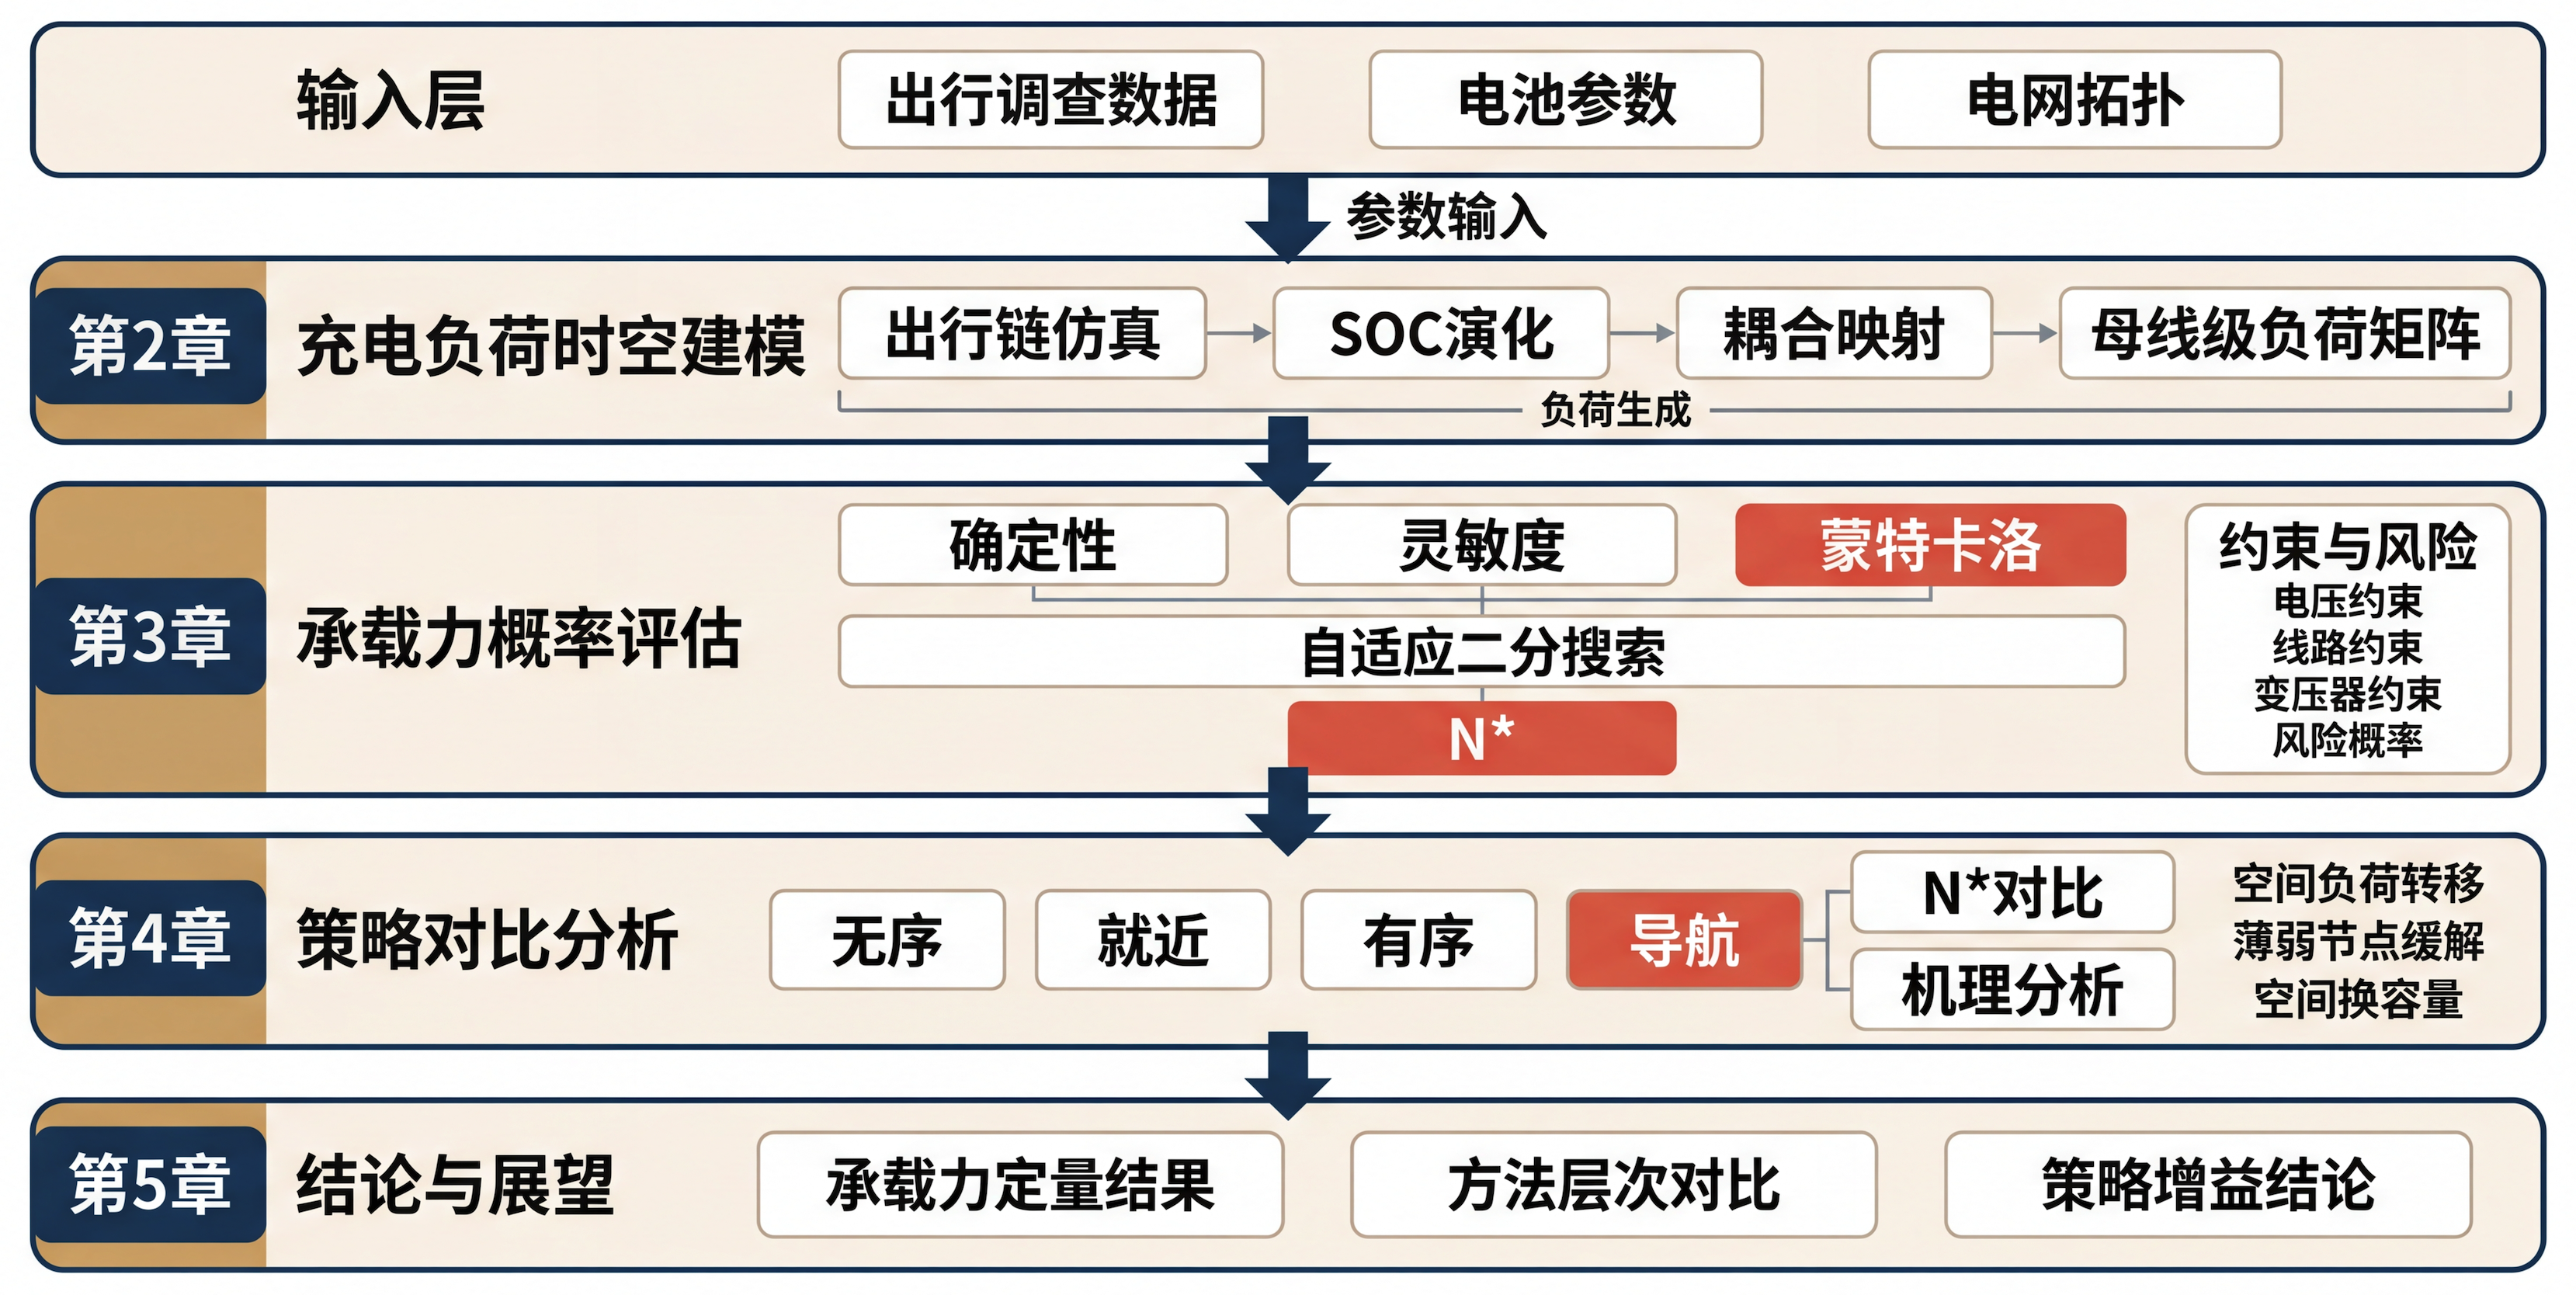
\includegraphics[width=0.9\textwidth]{1-2.png}
        \caption{本文研究框架}
        \label{fig:framework}
    \end{figure}

    \newpage
    \section{电动汽车充电负荷时空建模}
    \markboth{\text{第}\thesection\text{章} \quad 电动汽车充电负荷时空建模}{\text{第}\thesection\text{章} \quad 电动汽车充电负荷时空建模}

    充电负荷的准确建模是配电网承载力评估的前提与基础。本章构建基于出行链的电动汽车充电负荷时空仿真模型，完整刻画日内多次出行、驻留、充电全过程。首先阐述出行链的基本结构与各环节关键参数的概率分布设定，设计多日连续仿真框架以克服单日仿真的跨午夜截断缺陷；其次建立 SOC 状态演化方程与“下一程能量储备”充电触发判据；再通过交通、电力耦合映射机制将车辆充电需求投射至配电网母线，形成母线级时序充电负荷矩阵；最后实现会话式模型作为对比基线，并对两种模型的充电负荷特性进行分析。

    \subsection{出行链模型构建}

    \subsubsection{出行链基本结构}

    出行链方法将电动汽车日内活动描述为“出行、驻留”交替的完整序列，能够在统一框架下刻画用户从早间出发到夜间归家的全过程。与仅考虑单次充电事件的统计概率法相比，出行链方法的核心优势在于保留了日内多次出行的时空分散特征，使得充电负荷在时间分布和空间定位上更为贴近实际[9]。

    本文参考陈丽丹等[9]和李含玉等[10]的建模框架，将电动汽车日内活动划分为以下类型：家庭停留（Home, H）、工作停留（Work, W）和其他活动停留（Other, O，涵盖购物、餐饮、社交等）。日内出行链的基本结构为：

    \begin{equation}
    \label{eq:tripchain_structure}
    \text{H} \xrightarrow{\text{通勤}} \text{W} \xrightarrow{\text{出行}_1} \text{O}_1 \xrightarrow{\text{出行}_2} \text{O}_2 \cdots \xrightarrow{\text{返程}} \text{H}
    \end{equation}

    其中，车辆于早间从家庭出发通勤至工作地点，工作结束后可能经过若干中间停靠点（购物、餐饮等），最终返回家庭。每次出行构成一条行程段（leg），连续的行程段与驻留环节共同组成日内出行链。

    每条出行链的构建涉及以下随机变量：首次出发时刻 $t_{\text{dep}}$、各行程段的行驶距离 $d_i$（$i=1,2,\ldots,n_{\text{leg}}$）、工作驻留时长 $\tau_{\text{work}}$、中间停靠次数 $n_{\text{other}}$ 以及各中间停靠驻留时长 $\tau_{\text{other},j}$（$j=1,2,\ldots,n_{\text{other}}$）。上述变量均通过概率分布独立采样，并施加时间顺序约束以确保出行链在时间轴上的逻辑自洽性，即前一环节的离开时刻不得晚于后一环节的到达时刻。

    \begin{figure}[htbp]
        \centering
        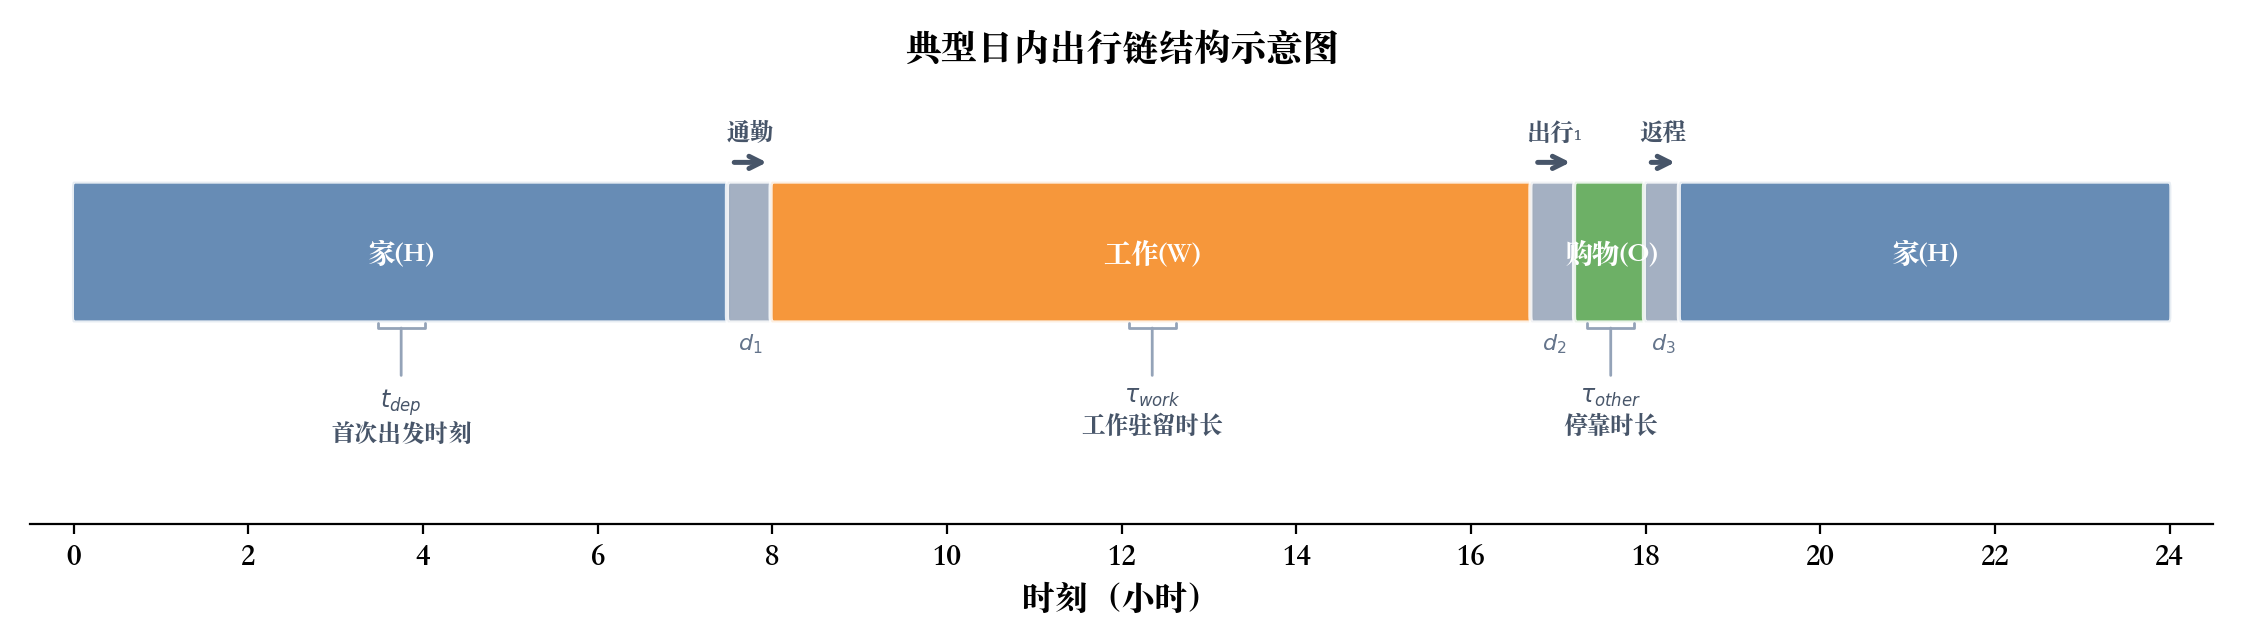
\includegraphics[width=0.90\textwidth]{fig_2_1.png}
        \caption{典型出行链结构示意图}
        \label{fig:trip_chain_structure}
    \end{figure}

    出行链中的每个驻留环节可形式化地定义为一个停靠点（Stop），其属性包括：所在区域编号 $z$、到达时刻 $t_{\text{arr}}$、离开时刻 $t_{\text{dep}}$ 和活动目的 $p$（取值为 home、work 或 other）。相邻停靠点之间的行程段具有行驶距离属性 $d$。一条完整的出行链可表示为停靠点的有序序列：

    \begin{equation}
    \label{eq:tripchain_formal}
    \mathcal{C} = \{(z_0, t_{\text{arr},0}, t_{\text{dep},0}, p_0),\ (z_1, t_{\text{arr},1}, t_{\text{dep},1}, p_1),\ \ldots,\ (z_m, t_{\text{arr},m}, t_{\text{dep},m}, p_m)\}
    \end{equation}

    其中 $m$ 为停靠点总数，需满足 $t_{\text{dep},i} \leq t_{\text{arr},i+1}$（$i=0,1,\ldots,m-1$），即时间单调递增约束。

    \subsubsection{关键参数的概率分布}

    出行链各环节的随机变量需要合理的概率分布加以刻画。本文参考国内外出行调查数据与已有文献的校准结果，对各参数分布进行如下设定。

    \noindent\textbf{（1）首次出发时刻}

    首次出发时刻 $t_{\text{dep}}$ 反映通勤出行的早间规律，采用正态分布描述：

    \begin{equation}
    \label{eq:dep_time_dist}
    t_{\text{dep}} \sim \mathcal{N}(\mu_t,\ \sigma_t^2)
    \end{equation}

    其中 $\mu_t$ 为均值（对应通勤早高峰中心时刻），$\sigma_t$ 为标准差（反映出发时间的离散程度）。本文取 $\mu_t = 7\text{:}30$（即 450 分钟）、$\sigma_t = 35$ 分钟。该设定与陈丽丹等[9]基于出行链的建模参数一致，同时对采样结果施加 $[0, 1440)$ 分钟的截断约束以确保物理合理性。

    \noindent\textbf{（2）日行驶里程}

    各行程段的行驶距离 $d$ 采用对数正态分布描述：

    \begin{equation}
    \label{eq:dist_lognormal}
    d \sim \text{LogNormal}(\mu_d,\ \sigma_d^2)
    \end{equation}

    对数正态分布的选取依据在于：行驶距离为正值且呈右偏分布，多数出行距离较短而少数长距离出行拉高尾部，这一特征与田立亭等[7]基于 NHTS 数据的统计结论一致。本文通过矩匹配方法将原始尺度的均值和标准差转换为对数尺度参数。设原始尺度均值为 $\bar{d}$、标准差为 $s_d$，则对数尺度参数为：

    \begin{equation}
    \label{eq:lognormal_params}
    \mu_d = \ln\frac{\bar{d}^2}{\sqrt{s_d^2 + \bar{d}^2}}, \quad \sigma_d = \sqrt{\ln\left(1 + \frac{s_d^2}{\bar{d}^2}\right)}
    \end{equation}

    本文取 $\bar{d} = 20$ km、$s_d = 10$ km，对应单程通勤距离的典型水平。

    \noindent\textbf{（3）工作驻留时长}

    工作驻留时长 $\tau_{\text{work}}$ 采用截断正态分布描述：

    \begin{equation}
    \label{eq:work_duration_dist}
    \tau_{\text{work}} \sim \mathcal{N}(\mu_w,\ \sigma_w^2), \quad \tau_{\text{work}} \geq 0
    \end{equation}

    本文取 $\mu_w = 520$ 分钟（约 8 小时 40 分钟）、$\sigma_w = 45$ 分钟，反映标准工作日的上班时间及其波动。

    \noindent\textbf{（4）中间停靠次数}

    工作结束后的中间停靠次数 $n_{\text{other}}$ 采用泊松分布描述：

    \begin{equation}
    \label{eq:other_stops_dist}
    n_{\text{other}} \sim \text{Poisson}(\lambda_{\text{other}})
    \end{equation}

    本文取 $\lambda_{\text{other}} = 1.0$，即每日平均一次中间停靠。该参数的选取综合考虑了陈丽丹等[9]给出的日均出行链长度（平均 3.02 段行程）以及典型私家车的日内活动模式。

    \noindent\textbf{（5）中间停靠驻留时长}

    中间停靠的驻留时长 $\tau_{\text{other}}$ 采用截断正态分布描述：

    \begin{equation}
    \label{eq:other_duration_dist}
    \tau_{\text{other}} \sim \mathcal{N}(\mu_o,\ \sigma_o^2), \quad \tau_{\text{other}} \geq 0
    \end{equation}

    本文取 $\mu_o = 50$ 分钟、$\sigma_o = 25$ 分钟，对应购物、餐饮等短时停靠的典型时长。

    \noindent\textbf{（6）行驶时间}

    各行程段的行驶时间由行驶距离与平均行驶速度换算得到：

    \begin{equation}
    \label{eq:travel_time}
    \tau_{\text{travel},i} = d_i \cdot \alpha
    \end{equation}

    其中 $\alpha$ 为单位里程行驶时间（分钟/km），本文取 $\alpha = 1.8$ 分钟/km，对应约 33 km/h 的城市综合平均车速。该换算关系在保持模型简洁性的同时，合理反映了城市工况下含路口信号灯和拥堵延迟的行驶速度水平。

    \begin{figure}[htbp]
        \centering
        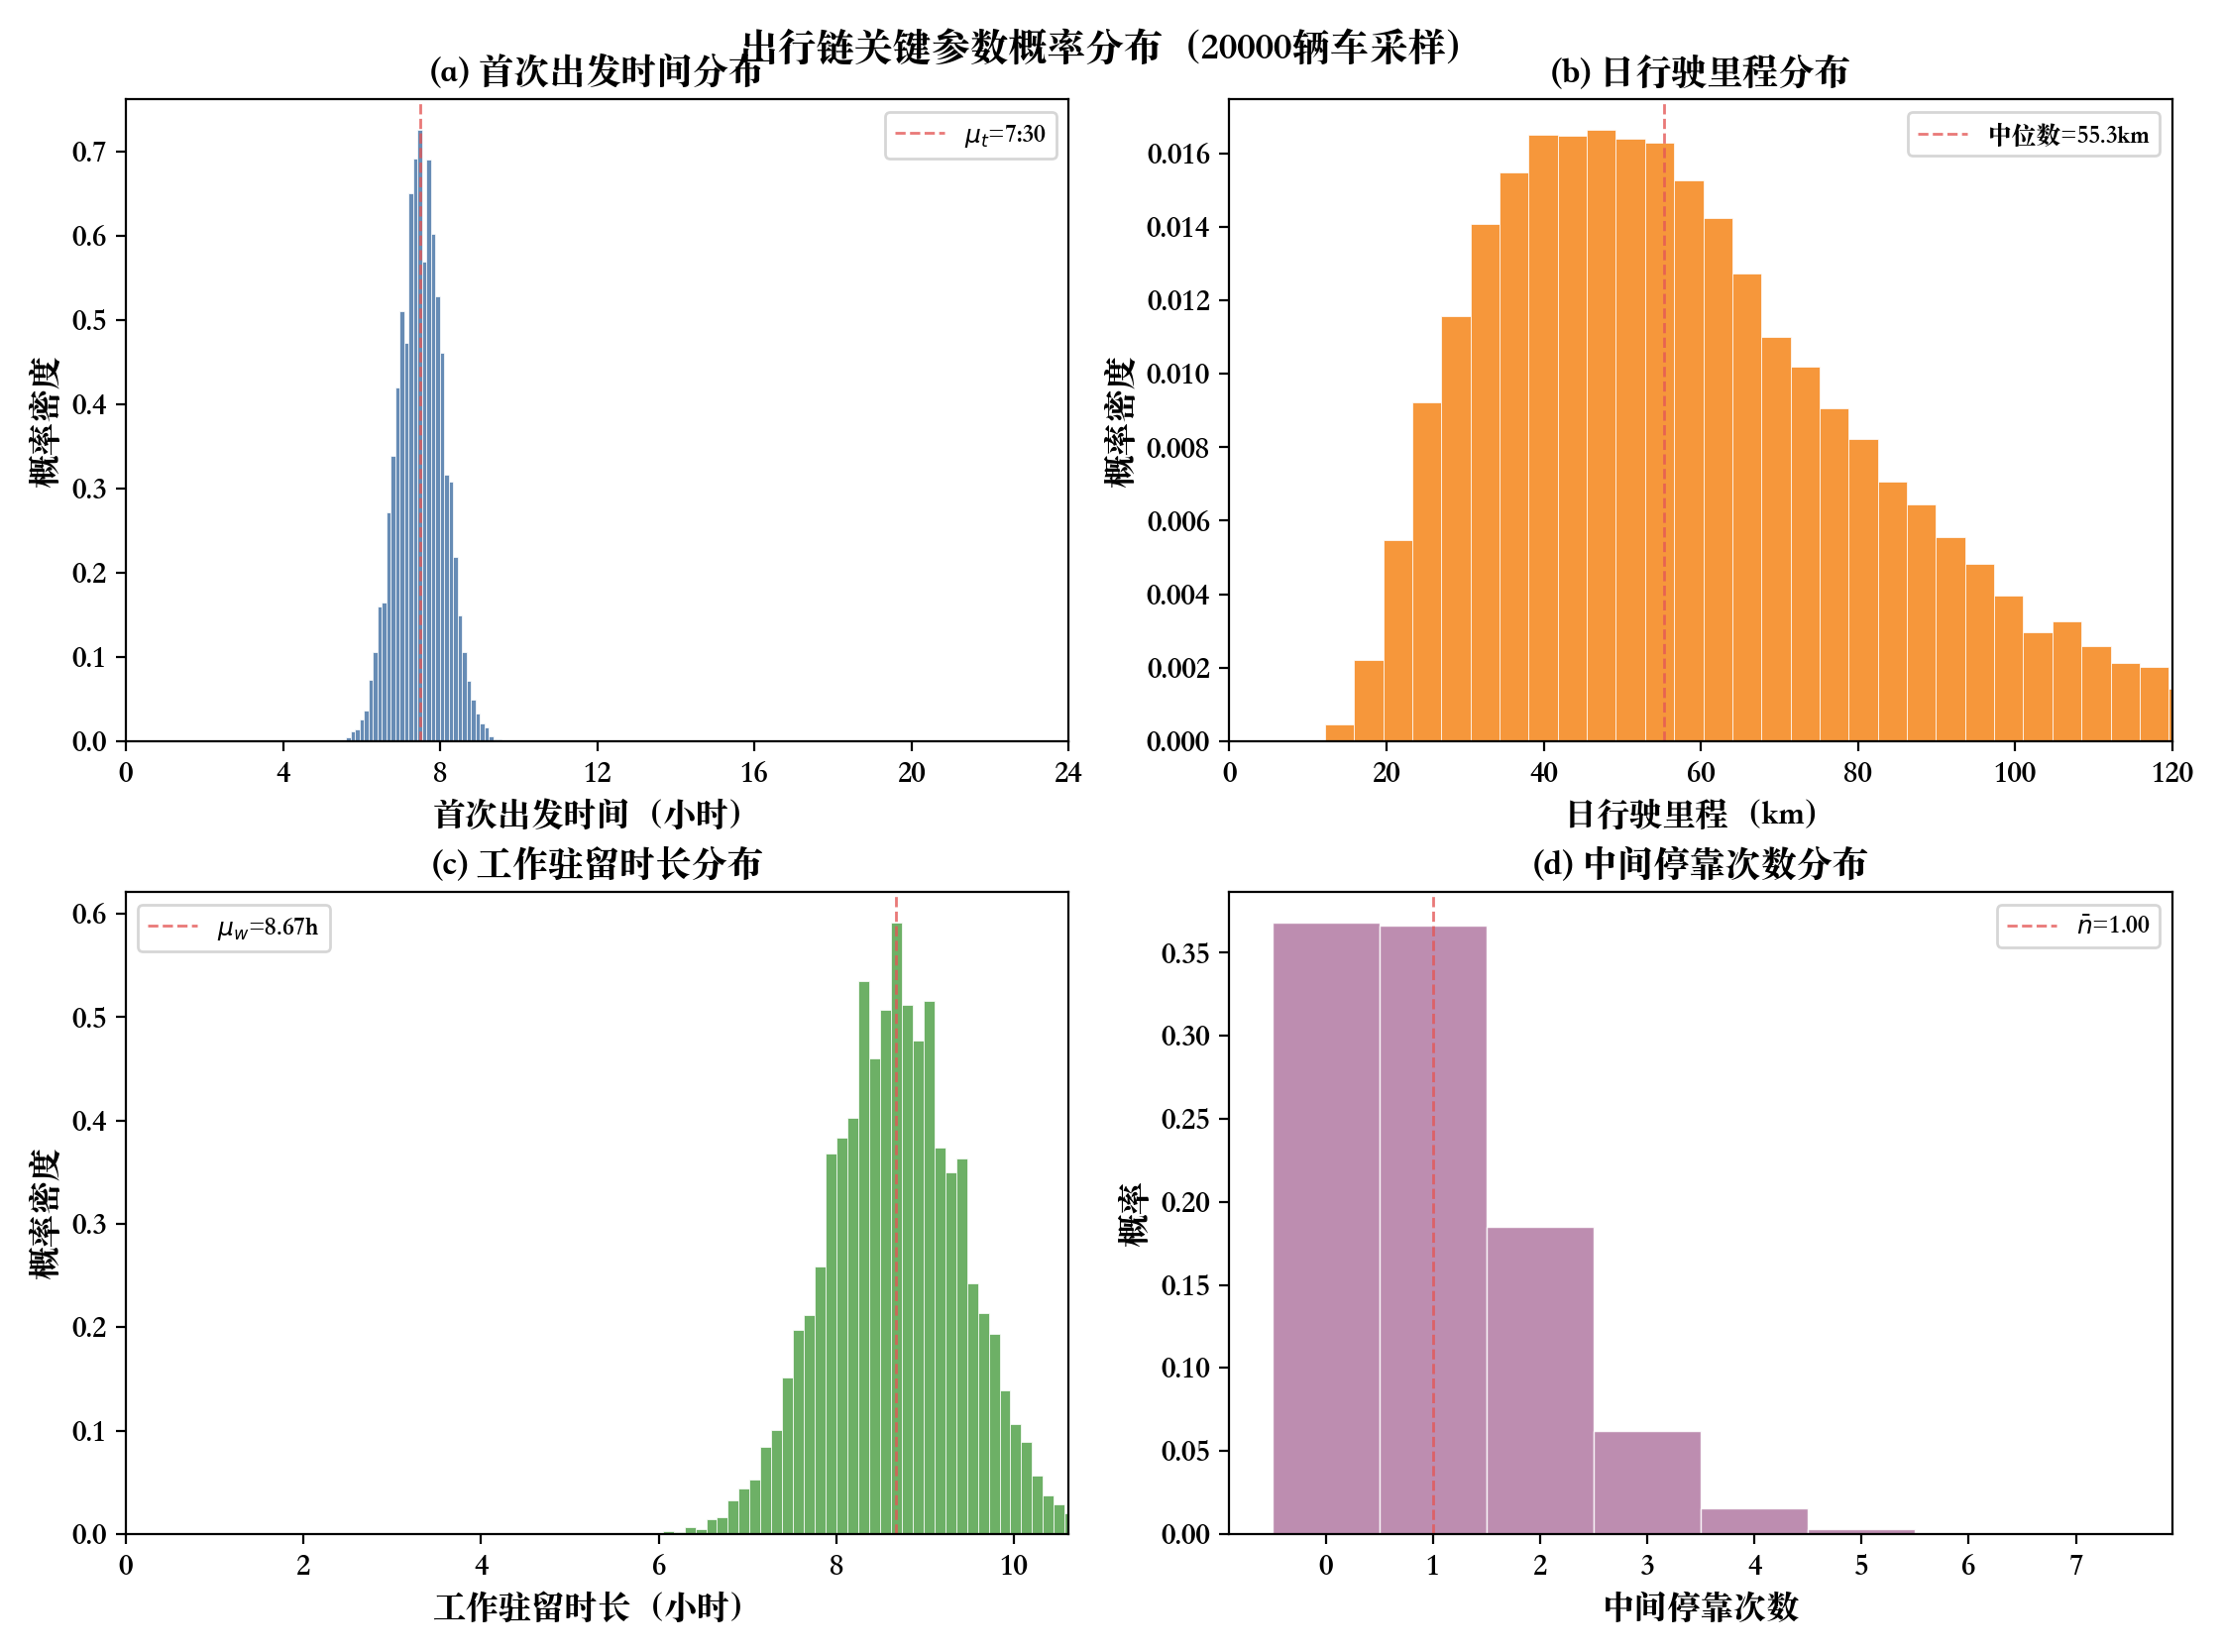
\includegraphics[width=0.82\textwidth]{fig_2_2.png}
        \caption{出行链关键参数概率分布（20000 辆车采样）}
        \label{fig:trip_chain_distribution}
    \end{figure}

    上述参数的取值汇总于表 \ref{tab:trip_chain_params}。

    \begin{table}[htbp]
        \centering
        \caption{出行链模型参数设定}
        \label{tab:trip_chain_params}
        \zihao{5}
        \setlength{\tabcolsep}{4pt}
        \renewcommand{\arraystretch}{1.3}
        \begin{tabular}{>{\raggedright\arraybackslash}p{3.0cm} >{\centering\arraybackslash}p{1.9cm} >{\centering\arraybackslash}p{2.8cm} >{\centering\arraybackslash}p{2.6cm} >{\centering\arraybackslash}p{1.5cm}}
            \toprule
            参数名称 & 符号 & 取值 & 分布类型 & 文献来源 \\
            \midrule
            首次出发时刻均值 & $\mu_t$ & 07:30（450 min） & 正态分布 & [9] \\
            首次出发时刻标准差 & $\sigma_t$ & 35 min & 正态分布 & [9] \\
            行驶距离均值 & $\bar{d}$ & 20 km & 对数正态分布 & [7][8] \\
            行驶距离标准差 & $s_d$ & 10 km & 对数正态分布 & [7][8] \\
            工作驻留时长均值 & $\mu_w$ & 520 min & 截断正态分布 & [9][10] \\
            工作驻留时长标准差 & $\sigma_w$ & 45 min & 截断正态分布 & [9][10] \\
            中间停靠次数 & $\lambda_{\text{other}}$ & 1.0 & 泊松分布 & [9] \\
            中间停靠驻留时长均值 & $\mu_o$ & 50 min & 截断正态分布 & [9] \\
            中间停靠驻留时长标准差 & $\sigma_o$ & 25 min & 截断正态分布 & [9] \\
            单位里程行驶时间 & $\alpha$ & 1.8 min/km & 确定性换算 & [4] \\
            交通区域数量 & $n_{\text{zone}}$ & 50 & --- & [4] \\
            \bottomrule
        \end{tabular}
    \end{table}

    \subsubsection{多日连续仿真框架}

    现有出行链模型多采用单日仿真框架，即在 $[0, 24\text{h})$ 的时间窗内完成所有出行与充电行为的模拟。然而，单日仿真存在一个关键缺陷：当有序充电策略将充电行为推迟至夜间低谷时段（如 22:00—次日 06:00）时，单日仿真在午夜截断，车辆仅有 2 小时的充电窗口（22:00—24:00），无法完成完整的充电过程。这一截断问题导致有序充电策略的效果被严重低估。

    为克服上述缺陷，本文设计了多日连续仿真框架。其核心思想为：逐日独立采样出行链，通过时间偏移拼接形成跨越多日的连续时间轴，使 SOC 状态和充电会话能够自然跨越午夜延续。

    具体实现步骤如下：

    \noindent\textbf{（1）逐日独立采样。}
    对每辆车的每一仿真日，独立调用出行链采样函数生成当日的出行序列。家庭区域和工作区域在仿真期间保持不变，以反映同一用户的固定通勤模式。

    \noindent\textbf{（2）时间偏移拼接。}
    第 $k$ 天（$k=0,1,\ldots,n_{\text{day}}-1$）的出行链中所有时间标记偏移 $k \times T_{\text{day}}$ 分钟，其中 $T_{\text{day}}$ 为单日仿真步长总时长。本文取 $T_{\text{day}} = 1440$ 分钟（24 小时），仿真天数 $n_{\text{day}} = 2$，故总仿真时长为 2880 分钟（48 小时），对应 192 个时步（每步 15 分钟）。

    \noindent\textbf{（3）跨午夜停留合并。}
    当第 $k$ 天出行链的末尾停靠与第 $k+1$ 天出行链的起始停靠位于同一区域且目的相同时（典型情况为夜间在家停留），将两个停靠合并为一个连续停留段。合并后，该停留段的时间窗跨越午夜边界，允许充电会话在夜间完整执行。当末尾停靠与起始停靠不在同一区域时，插入零距离边界行程段以维持时间轴的连续性。

    \begin{figure}[htbp]
        \centering
        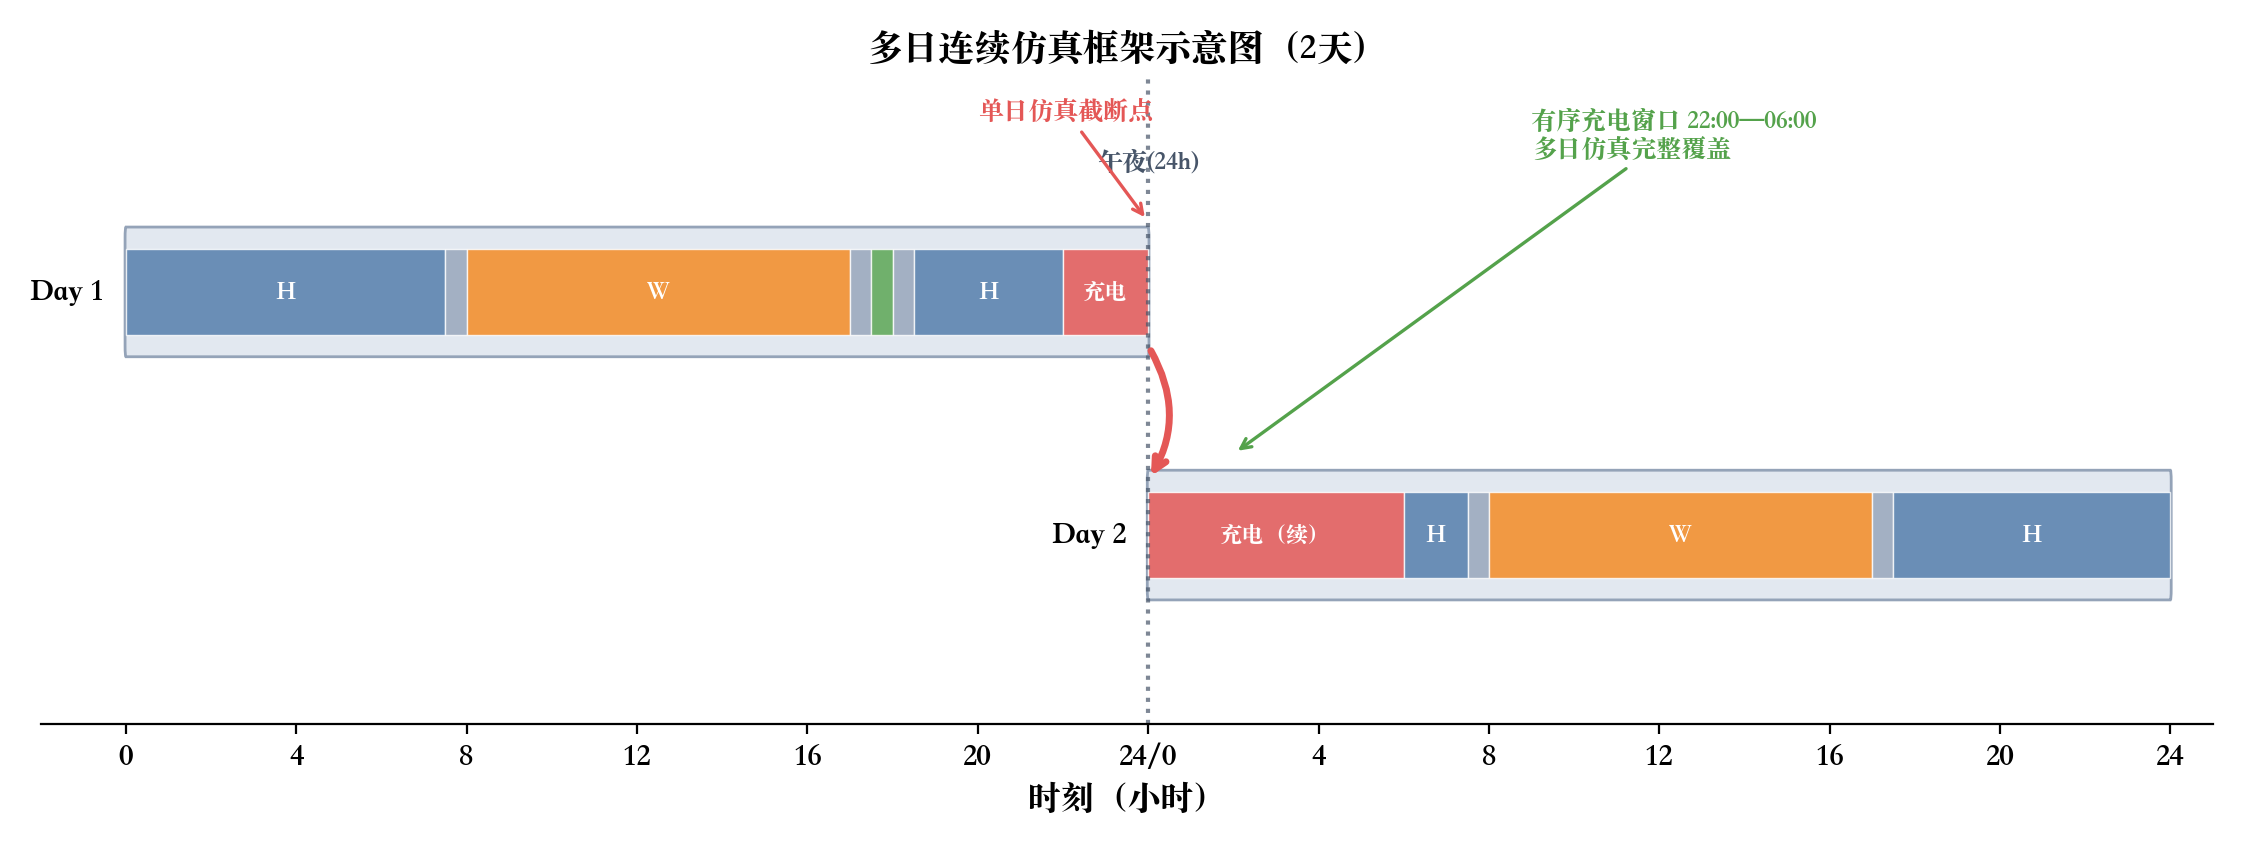
\includegraphics[width=0.86\textwidth]{fig_2_3.png}
        \caption{多日连续仿真框架示意图（2 天）}
        \label{fig:multi_day_framework}
    \end{figure}

    多日连续仿真框架的引入带来两方面改进：一是在多日模式下，仿真起始时刻（第 0 天的 0:00）车辆处于家中停靠状态，该初始停靠点也被设置为可触发充电，从而模拟真实场景中车辆在仿真起始前可能已处于充电状态的情况；二是跨午夜充电会话的完整覆盖使得有序充电策略的效果评估更为准确，避免了单日仿真对夜间充电窗口的人为截断。

    \subsection{SOC演化与充电决策模型}

    \subsubsection{SOC状态演化方程}

    电动汽车的荷电状态（State of Charge, SOC）在日内出行过程中经历“行驶消耗、停靠充电”的交替演化。本文在 1 分钟的时间分辨率上模拟 SOC 的逐分钟变化，随后聚合至 15 分钟时步输出充电功率时序。

    行驶耗电模型。车辆在行程段 $i$ 的行驶过程中消耗电能 $\Delta E_{\text{drive},i}$：

    \begin{equation}
    \label{eq:energy_drive}
    \Delta E_{\text{drive},i} = \omega \cdot d_i
    \end{equation}

    其中 $\omega$ 为单位里程能耗（kWh/km），$d_i$ 为行程段 $i$ 的行驶距离（km）。本文取 $\omega = 0.18$ kWh/km，该取值参考了邵尹池等[4]给出的城市综合工况能耗水平（0.16—0.25 kWh/km）。在仿真实现中，行驶耗电在行程段的起止时间内均匀扣除。

    充电补能模型。车辆在停靠点充电时，电池储能逐分钟增加：

    \begin{equation}
    \label{eq:energy_charge}
    E_{t+1} = E_t + \eta \cdot P_{\text{ch}} \cdot \Delta t
    \end{equation}

    其中 $E_t$ 为 $t$ 时刻的电池储能（kWh），$\eta$ 为充电效率，$P_{\text{ch}}$ 为充电功率（kW），$\Delta t = 1/60$ 小时（1 分钟）。充电过程持续直至电池充满（$E = C$，$C$ 为电池额定容量）或车辆离开停靠点，取先到达者终止。

    SOC 离散递推。综合行驶消耗与充电补能，SOC 的离散递推方程为：

    \begin{equation}
    \label{eq:soc_recursion}
    \text{SOC}_{t+1} = \text{clip}\left(\frac{E_{t+1}}{C},\ \text{SOC}_{\min},\ \text{SOC}_{\max}\right)
    \end{equation}

    其中 $\text{SOC}_{\min} = 0$、$\text{SOC}_{\max} = 1$，$\text{clip}(\cdot)$ 函数将 SOC 限制在合理范围内。每个 15 分钟时步结束时记录 SOC 值，形成 SOC 时序曲线。

    充电功率输出。电网侧的充电功率为恒定值 $P_{\text{ch}}$（不考虑充电效率损耗），在每个 15 分钟时步内按充电分钟数占比进行平均：

    \begin{equation}
    \label{eq:avg_power}
    \bar{P}_k = P_{\text{ch}} \cdot \frac{n_{\text{charge},k}}{\Delta T}
    \end{equation}

    其中 $\bar{P}_k$ 为第 $k$ 个时步的平均充电功率，$n_{\text{charge},k}$ 为该时步内充电的分钟数，$\Delta T$ 为时步长度（15 分钟）。

    \subsubsection{充电触发判据}

    充电触发判据决定车辆在到达某个停靠点后是否启动充电。本文采用“下一程能量储备”判据，该判据的设计参考了陈丽丹等[9]提出的充电条件判断方法以及李含玉等[10]的改进方案。

    判据定义。车辆在到达停靠点 $n$ 时，若剩余电量不足以完成下一段行程并维持安全储备，则触发充电：

    \begin{equation}
    \label{eq:charge_trigger}
    E_n - \omega \cdot d_{n+1} < r \cdot C
    \end{equation}

    其中 $E_n$ 为到达停靠点 $n$ 时的电池储能（kWh），$d_{n+1}$ 为下一段行程的行驶距离（km），$r$ 为安全储备系数，$C$ 为电池额定容量（kWh）。本文取 $r = 0.3$，即要求完成下一段行程后 SOC 不低于 30\%。该阈值与陈丽丹等[9]给出的 30\% SOC 安全裕度一致。

    与简单 SOC 阈值判据的区别。传统的简单 SOC 阈值判据（如 SOC $< 30\%$ 时充电）仅基于当前 SOC 水平判断，而不考虑后续行程的能量需求。“下一程能量储备”判据的优势在于：当下一段行程较短时，即使当前 SOC 较低也可能无需充电；当下一段行程较长时，即使当前 SOC 较高也可能需要提前充电。这种前瞻性的判断机制更为合理地反映了驾驶员的实际充电决策行为[9][10]。

    充电地点约束。并非所有停靠点均具备充电条件。本文设定仅在家庭（home）和工作（work）类型的停靠点允许充电，这一假设基于当前充电基础设施的实际布局，即居住区和工作区是私家车慢充桩的主要安装场所。中间停靠点（如购物中心）由于驻留时间较短且公共充电桩覆盖率有限，暂不纳入可充电场所。

    末次居家补充充电规则。上述“下一程能量储备”判据仅在车辆剩余电量不足以安全完成下一段行程时才触发充电。然而在实际用车习惯中，车主在傍晚或夜间最终返家后往往会主动插枪充电，即使当前 SOC 足以应对次日出行。为刻画这一行为特征，本文在“下一程能量储备”判据之外补充设计了“末次居家补充充电”规则。

    首先定义当日末次家庭停靠：若停靠点目的为“家庭”，且该停靠点为出行链的最后一个停靠点，或该停靠点的停留时间跨越日边界（即到达日期与离开日期不同），则认定该停靠点为当日末次家庭停靠。

    其次，引入时间依赖的参与概率函数 $\rho(t)$ 刻画车主是否触发补充充电的意愿：

    \begin{equation}
    \label{eq:participation_prob}
    \rho(t) =
    \begin{cases}
        0, & t < 17\text{:}00 \\
        0.1 + 0.9 \cdot \dfrac{t - 17\text{:}00}{22\text{:}00 - 17\text{:}00}, & 17\text{:}00 \leq t < 22\text{:}00 \\
        1.0, & 22\text{:}00 \leq t \text{ 或 } t < 06\text{:}00
    \end{cases}
    \end{equation}

    该概率函数的设计依据为：17:00 之前的家庭停留通常为午间临时返家，不宜视为日终充电；17:00 至 22:00 期间回家的车辆，其触发补充充电的意愿随时间线性递增（从 10\% 增至 100\%）；22:00 之后及次日凌晨 06:00 之前到达的车辆，均被视为日终停靠，以概率 1 触发充电。

    当末次居家补充充电被触发时，其充电目标 SOC 设为 $\text{SOC}_{\text{home}} = 0.9$（低于充满状态 1.0），反映实际场景中车主“充至八九成即可”的行为习惯。充电规则的完整判断逻辑为：若“下一程能量储备”判据已触发，则充电目标取 $\text{SOC}_{\max}$（即充满）；若仅末次居家补充规则触发（以概率 $\rho(t)$ 采样决定），则充电目标取 $\text{SOC}_{\text{home}}$。两条判据取并集，确保不遗漏任何一种充电需求。

    该规则的引入使模型更贴近实际充电行为：在傍晚至夜间高峰时段，大量车辆即使 SOC 尚充裕仍会触发家庭充电，形成更为真实的晚高峰充电负荷峰值；而在非高峰时段返家的车辆则以较低概率充电，体现了行为异质性。

    充电时长计算。当充电被触发时，充电从当前 SOC 到目标 SOC 所需的时长为：

    \begin{equation}
    \label{eq:charge_duration}
    T_{\text{charge}} = \left\lceil\frac{(\text{SOC}_{\text{target}} - \text{SOC}_{\text{arr}}) \cdot C}{\eta \cdot P_{\text{ch}}} \times 60\right\rceil \text{（分钟）}
    \end{equation}

    其中 $\text{SOC}_{\text{arr}}$ 为到达时的 SOC，$\text{SOC}_{\text{target}}$ 为充电目标 SOC（由“下一程能量储备”判据触发时取 $\text{SOC}_{\max} = 1$，由“末次居家补充”规则触发时取 $\text{SOC}_{\text{home}} = 0.9$），$\lceil\cdot\rceil$ 为向上取整。实际充电时长为 $\min(T_{\text{charge}},\ t_{\text{dep}} - t_{\text{arr}})$，即不超过停靠时间窗。

    \begin{figure}[htbp]
        \centering
        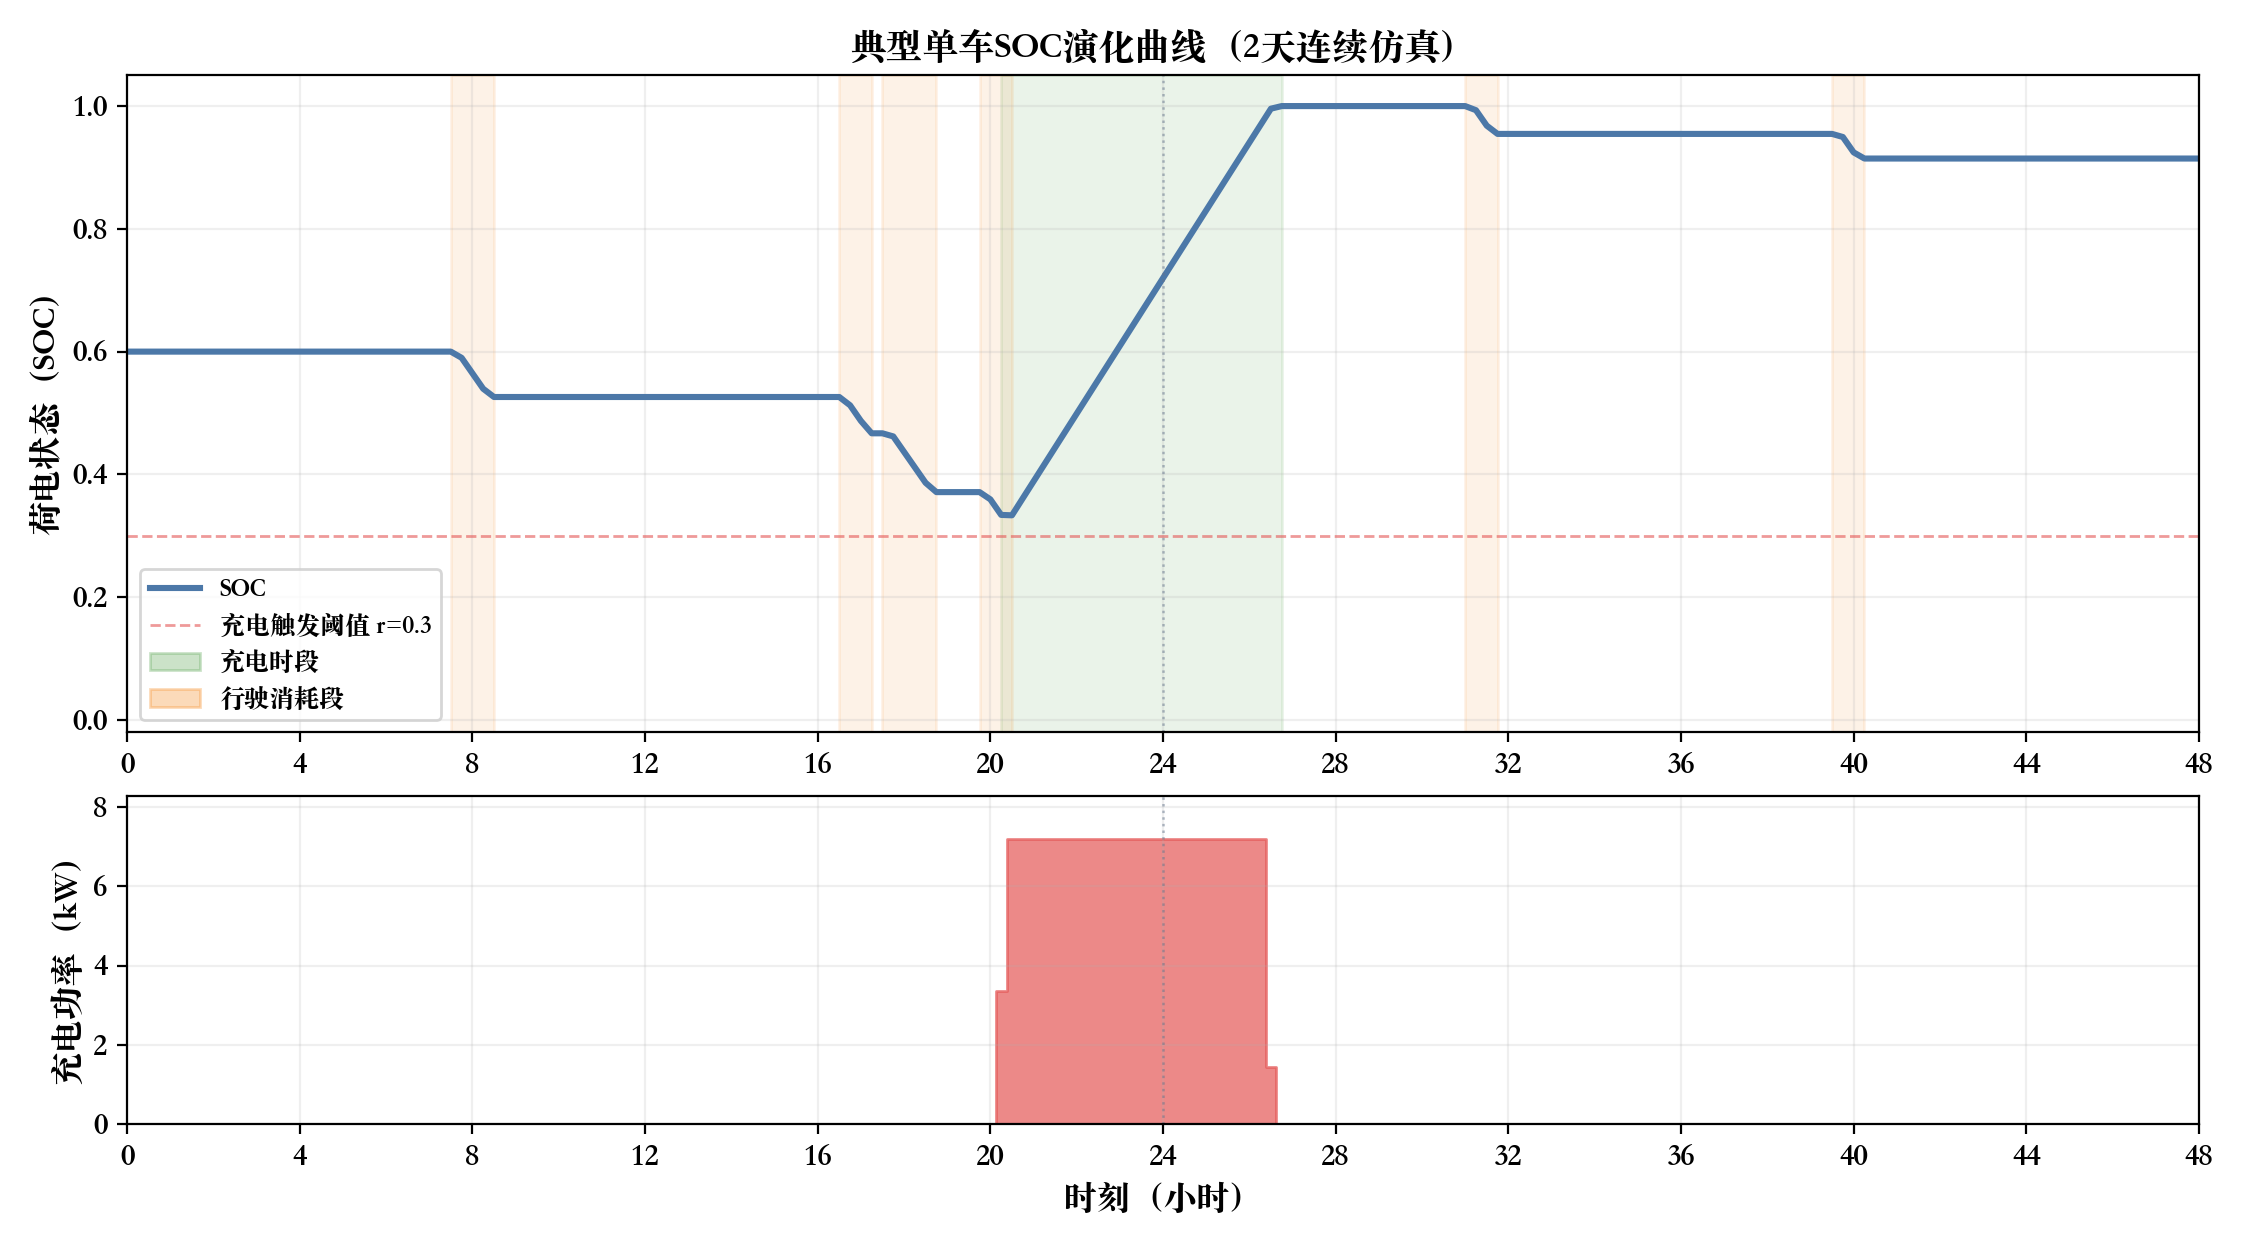
\includegraphics[width=0.82\textwidth]{fig_2_4.png}
        \caption{典型单车 SOC 演化曲线（2 天连续仿真）}
        \label{fig:soc_evolution}
    \end{figure}

    \subsubsection{车辆与电池基本参数}

    本文的仿真对象为典型私家车型电动汽车，电池与充电相关参数的设定综合参考了多篇文献的取值。电池额定容量取 60 kWh，对应当前主流纯电动汽车的电池配置水平；慢充功率取 7.2 kW，为家用交流慢充桩的典型功率等级；充电效率取 0.92，考虑了交流、直流变换和电池内阻的综合损耗。

    初始 SOC 采用截断正态分布描述：

    \begin{equation}
    \label{eq:init_soc_dist}
    \text{SOC}_0 \sim \mathcal{N}(\mu_{\text{SOC}},\ \sigma_{\text{SOC}}^2), \quad \text{SOC}_0 \in [0, 1]
    \end{equation}

    本文取 $\mu_{\text{SOC}} = 0.60$、$\sigma_{\text{SOC}} = 0.10$。初始 SOC 均值的选取参考了罗卓伟等[8]给出的私家车初始 SOC 分布 $\mathcal{N}(0.6, 0.1^2)$，反映了私家车日间出行后的典型电量水平。

    \begin{table}[htbp]
        \centering
        \caption{电动汽车与电池模型参数}
        \label{tab:ev_battery_params}
        \zihao{5}
        \setlength{\tabcolsep}{4pt}
        \renewcommand{\arraystretch}{1.3}
        \begin{tabular}{>{\raggedright\arraybackslash}p{3.0cm} >{\centering\arraybackslash}p{2.0cm} >{\centering\arraybackslash}p{2.2cm} >{\centering\arraybackslash}p{1.8cm} >{\centering\arraybackslash}p{2.0cm}}
            \toprule
            参数 & 符号 & 取值 & 单位 & 来源 \\
            \midrule
            电池额定容量 & $C$ & 60 & kWh & 综合设定 \\
            慢充功率 & $P_{\text{ch}}$ & 7.2 & kW & [7][8] \\
            充电效率 & $\eta$ & 0.92 & --- & [9] \\
            单位里程能耗 & $\omega$ & 0.18 & kWh/km & [4] \\
            初始 SOC 均值 & $\mu_{\text{SOC}}$ & 0.60 & --- & [8] \\
            初始 SOC 标准差 & $\sigma_{\text{SOC}}$ & 0.10 & --- & [8] \\
            SOC 安全储备系数 & $r$ & 0.30 & --- & [9] \\
            末次居家补充充电 & --- & 启用 & --- & 本文 \\
            补充充电目标 SOC & $\text{SOC}_{\text{home}}$ & 0.90 & --- & 本文 \\
            仿真时步 & $\Delta T$ & 15 & min & [3] \\
            仿真天数 & $n_{\text{day}}$ & 2 & 天 & 本文 \\
            SOC 仿真分辨率 & --- & 1 & min & [10] \\
            \bottomrule
        \end{tabular}
    \end{table}

    \subsection{交通与电力耦合映射机制}

    出行链模型生成的充电需求发生在交通网络的各个区域中，而承载力评估需要将充电负荷定位至配电网的具体母线上。为此，需要建立交通区域与配电网母线之间的耦合映射关系。

    邵尹池等[4]在“车-路-网”建模框架中提出了路网节点与配电网节点的空间耦合映射方法，通过地理邻近关系将交通网络中各区域的充电需求分配至对应的配电网母线。本文借鉴该思想，建立映射函数 $\varphi: \mathcal{Z} \rightarrow \mathcal{B}$，将交通区域集合 $\mathcal{Z} = \{1, 2, \ldots, n_{\text{zone}}\}$ 映射至配电网母线集合 $\mathcal{B} = \{b_1, b_2, \ldots, b_{n_{\text{bus}}}\}$。

    映射矩阵表示。映射关系通过概率矩阵 $\mathbf{M} \in \mathbb{R}^{n_{\text{zone}} \times n_{\text{bus}}}$ 表示，其中 $M_{ij}$ 为交通区域 $i$ 的充电需求分配至母线 $j$ 的权重。在确定性映射模式下，$\mathbf{M}$ 退化为 one-hot 矩阵，每个区域唯一对应一条母线。映射矩阵在仿真开始前基于系统拓扑确定并固定，不随场景变化。

    本文采用随机 one-hot 映射策略：在仿真初始化时，以均匀分布为每个交通区域随机分配一条配电网母线。该策略虽然简化了真实的交通、电力空间关系，但在缺乏实际 GIS 数据的情况下，能够合理模拟充电需求在母线间的随机分散特征。映射关系一经确定即保持不变，确保不同仿真场景之间的可比性。

    \begin{figure}[htbp]
        \centering
        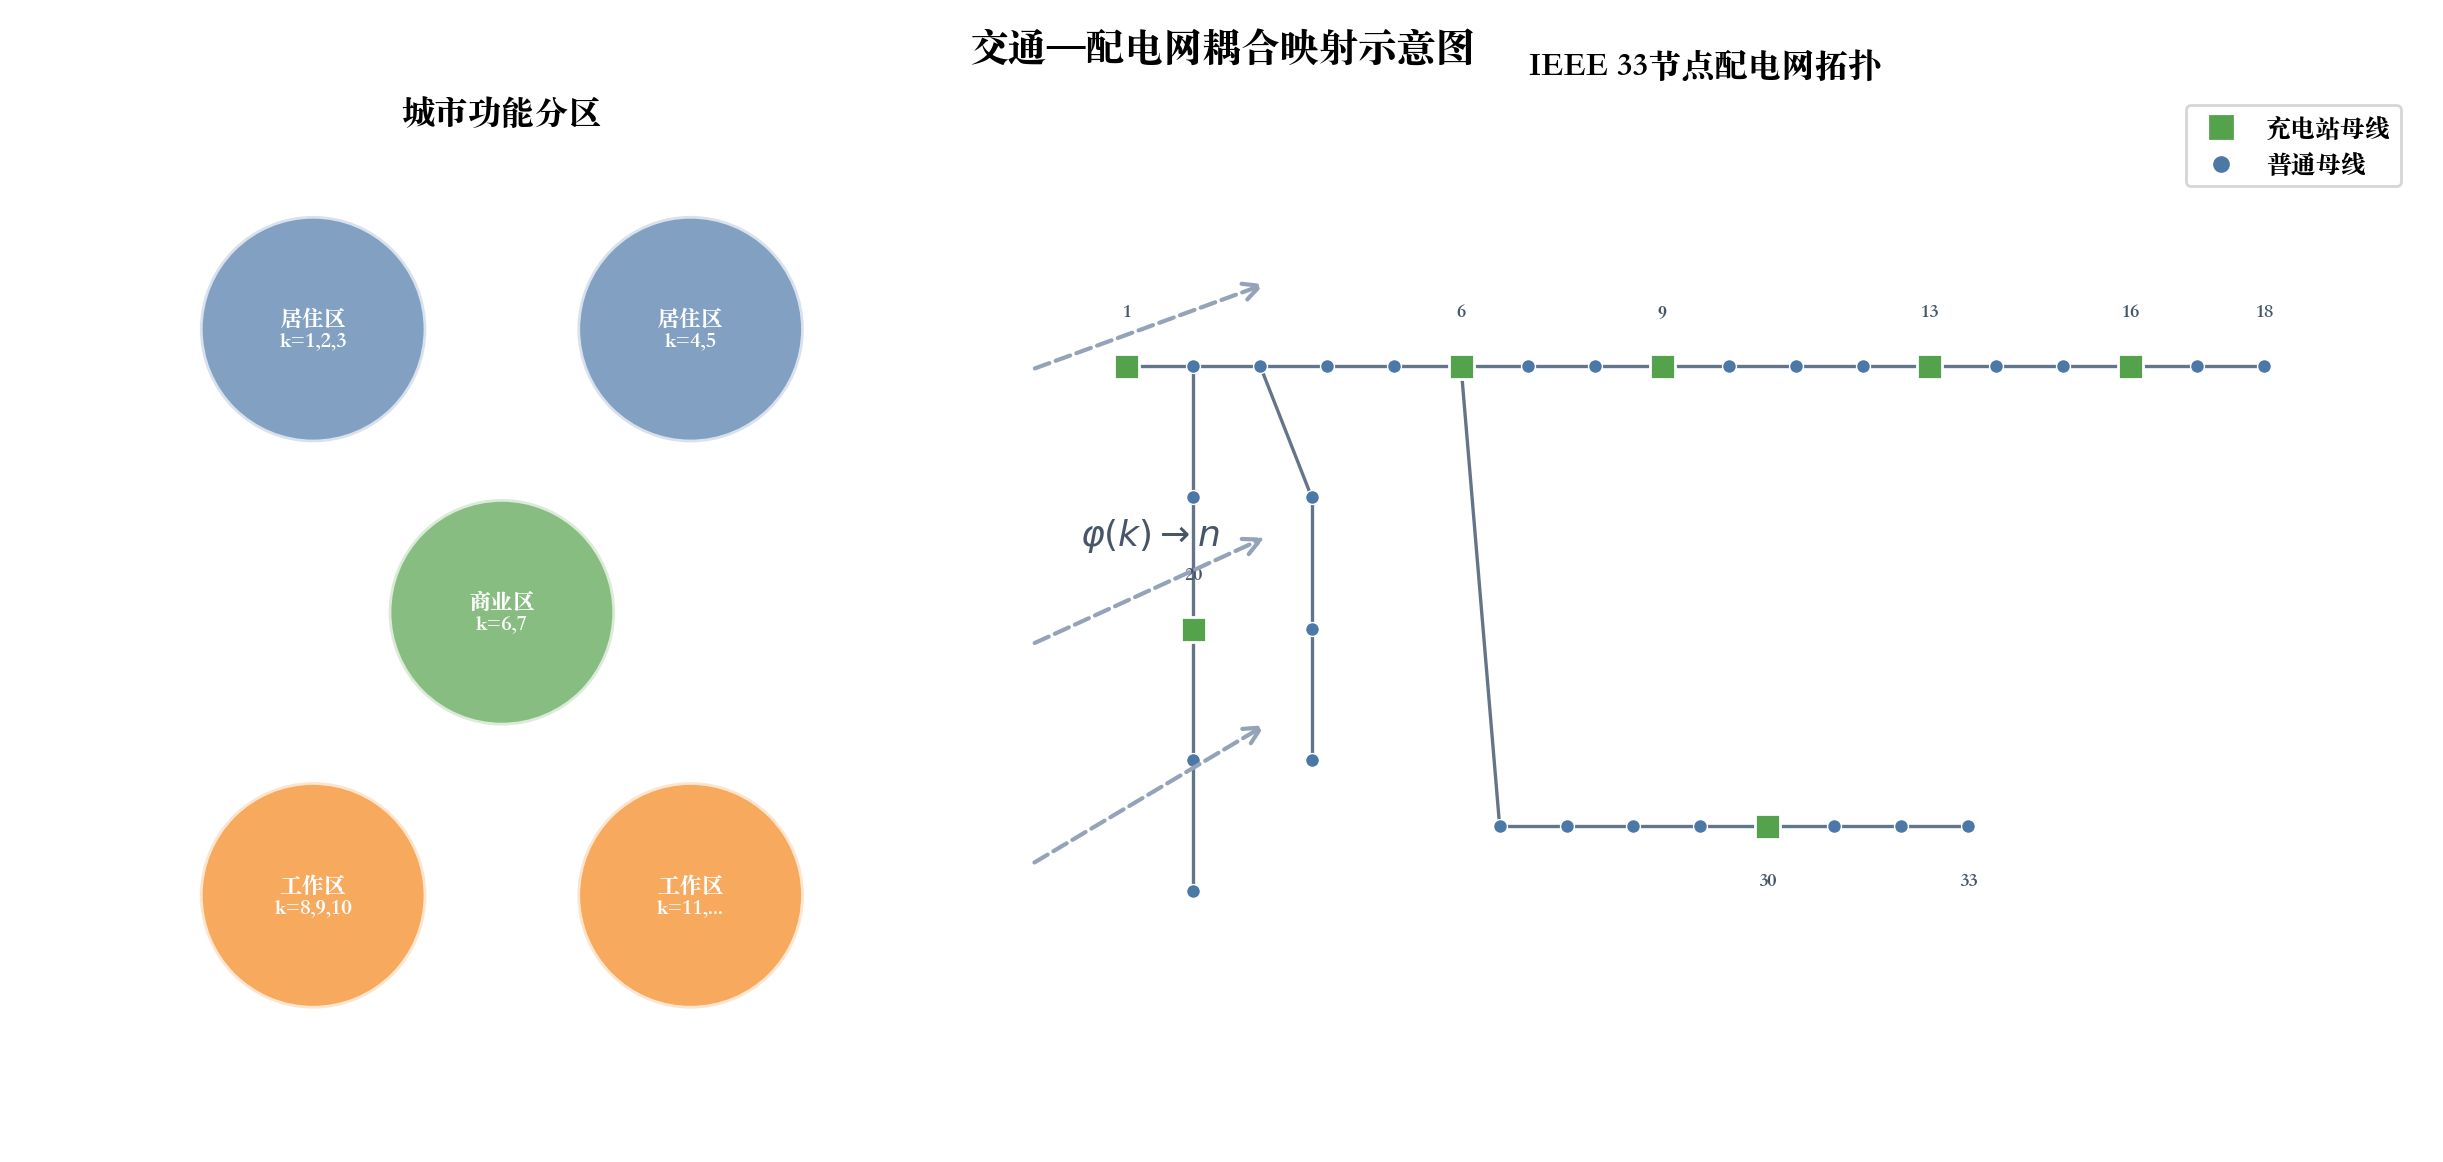
\includegraphics[width=0.86\textwidth]{fig_2_5.png}
        \caption{交通-配电网耦合映射示意图}
        \label{fig:traffic_power_mapping}
    \end{figure}

    充电站空间位置模型。对于需要空间策略（就近充电、充电导航）的仿真场景，本文引入黄梦旗等[17]文献中的 IEEE 33 节点系统充电站距离矩阵。该矩阵给出了 33 个配电网节点到 7 个充电站（分别位于母线 1、6、9、13、16、20、30）的距离数据，为充电导航策略中的距离衰减权重计算提供空间信息基础。

    母线级时序负荷矩阵构建。在映射关系确定后，每辆车的充电功率时序根据其停靠区域的映射关系投射至对应母线。$N$ 辆车的充电功率在各母线上逐时步叠加，形成母线级时序充电负荷矩阵 $\mathbf{P} \in \mathbb{R}^{T \times n_{\text{bus}}}$：

    \begin{equation}
    \label{eq:bus_load_matrix}
    P_{t,b} = \sum_{v=1}^{N} p_{v,t} \cdot \mathbf{1}[\varphi(z_{v,t}) = b]
    \end{equation}

    其中 $P_{t,b}$ 为第 $t$ 个时步母线 $b$ 上的聚合充电功率（MW），$p_{v,t}$ 为车辆 $v$ 在第 $t$ 个时步的充电功率，$z_{v,t}$ 为车辆 $v$ 在第 $t$ 个时步所处的交通区域，$\mathbf{1}[\cdot]$ 为示性函数。该矩阵是后续潮流计算和承载力评估的直接输入。

    \subsection{会话式模型（对比基线）}

    为系统评估出行链模型相较于传统方法在承载力评估中的差异，本文实现了会话式充电模型作为对比基线。会话式模型的建模思路源自田立亭等[7]的统计概率法，以充电起始时刻和充电持续时长为核心随机变量，每辆车每日产生若干独立的充电会话。

    充电起始时刻。采用混合正态分布描述用户充电行为的时间分散特征，主峰对应晚间归家后的充电时段：

    \begin{equation}
    \label{eq:session_start_time}
    t_{\text{start}} \sim \sum_{c=1}^{C} w_c \cdot \mathcal{N}(\mu_c,\ \sigma_c^2)
    \end{equation}

    其中各分量的权重 $w_c$、均值 $\mu_c$ 和标准差 $\sigma_c$ 根据配置参数设定。

    充电持续时长。采用截断正态分布描述，反映不同 SOC 水平下充电时长的差异。

    每日充电会话数。采用泊松分布描述每辆车每日的充电次数，均值参数 $\lambda$ 反映车辆的平均日充电频次。

    会话式模型的本质特征在于：它直接从充电事件的统计特性出发进行建模，而不刻画产生充电需求的出行行为细节。这一简化使其在充电负荷的时间分布和空间分布上与出行链模型存在系统性差异，即会话式模型的充电事件在时间上更为集中（缺乏日内多次出行的时间分散效应），在空间上更为随机（未建立出行活动与充电地点的因果关联）。这些差异将在第 4 章中体现为两种模型下承载力评估结果的显著不同。

    \subsection{充电负荷特性分析}

    基于上述模型，本节对大规模电动汽车聚合充电负荷的时序特性和空间分布特性进行分析。

    \noindent\textbf{（1）聚合充电负荷时序曲线}

    \begin{figure}[htbp]
        \centering
        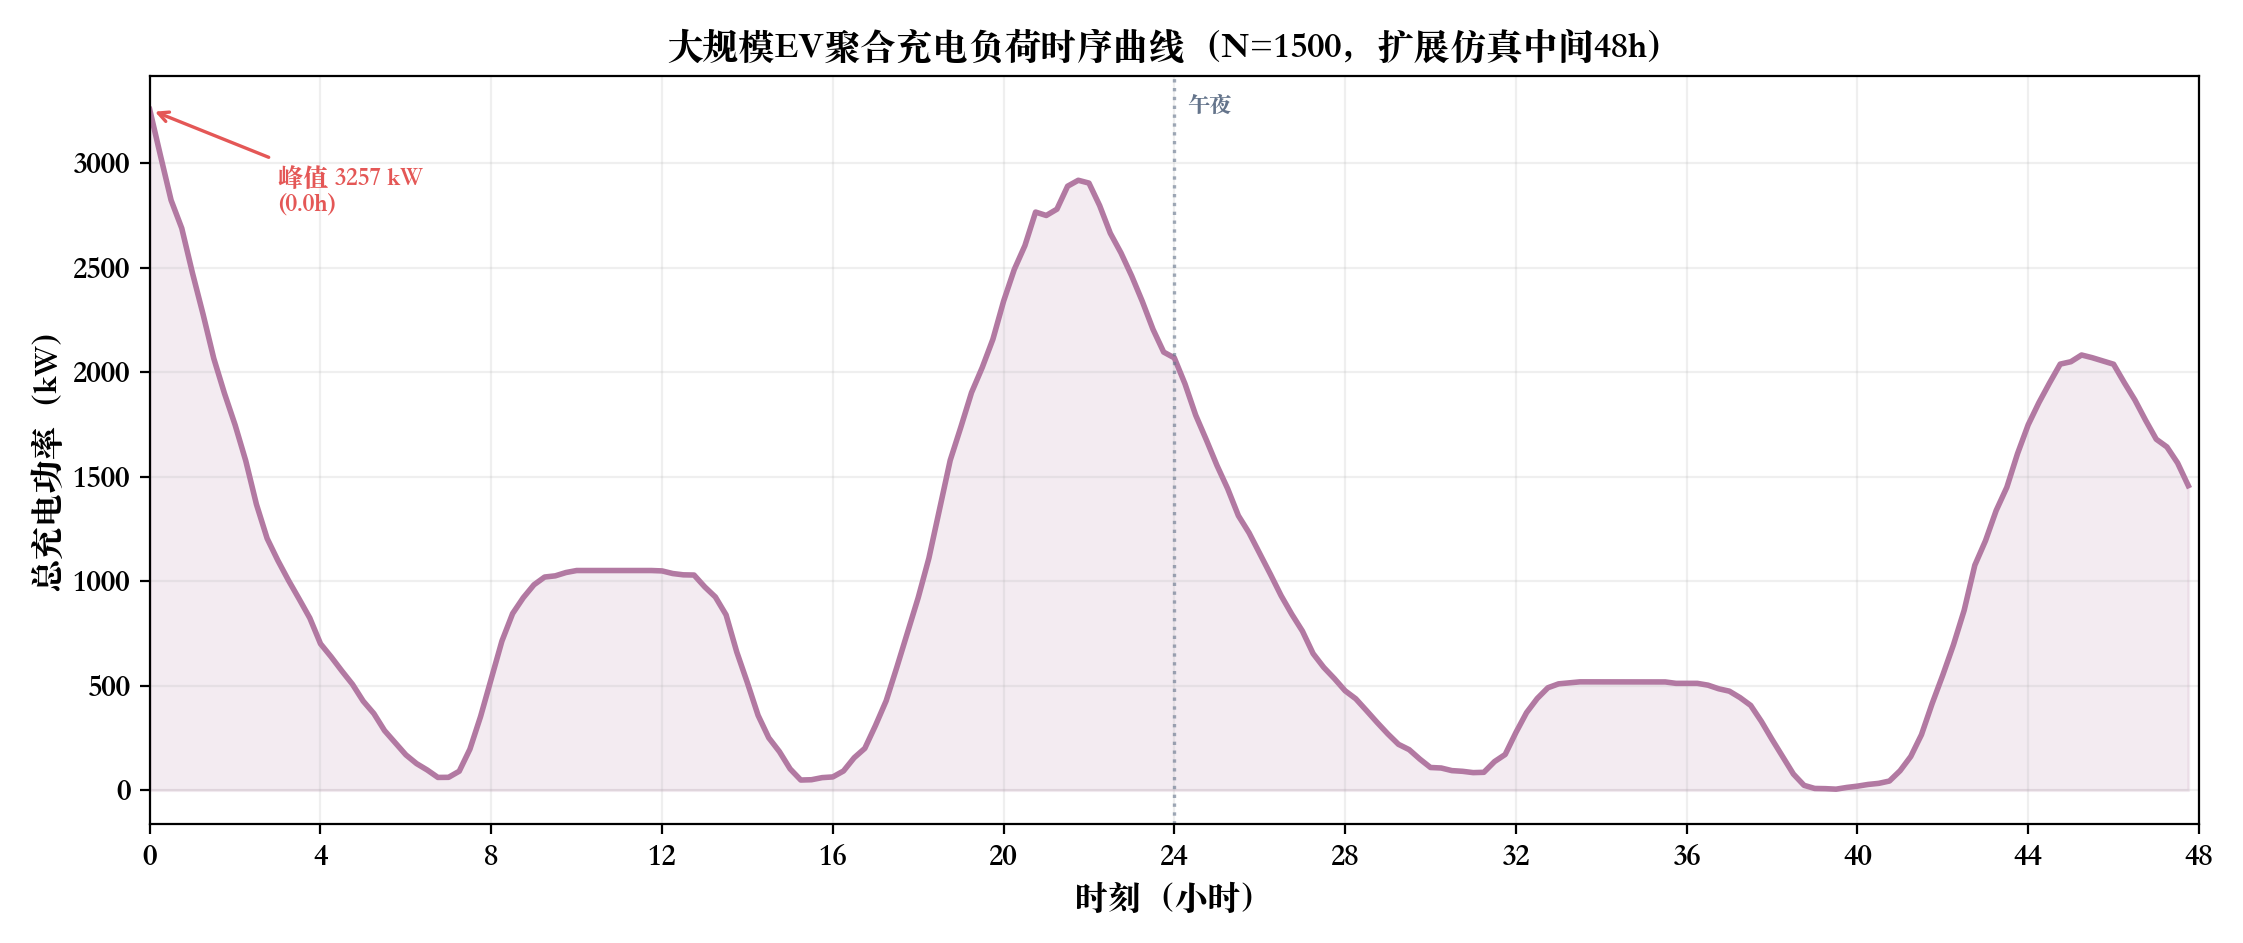
\includegraphics[width=0.86\textwidth]{fig_2_6.png}
        \caption{大规模 EV 聚合充电负荷时序曲线（$N = 1500$，扩展仿真截取中间 48 h）}
        \label{fig:aggregate_load_curve}
    \end{figure}

    在出行链模型的无序充电模式下，聚合充电负荷呈现出明显的时间规律性。由于大部分车辆在工作日下班后归家启动充电，充电负荷的峰值主要出现在 18:00—24:00 时段，与居民用电晚高峰高度重合，形成“峰上加峰”效应。为减弱仿真起始时刻初始 SOC 和仿真终止时刻末端截断对曲线形态的扰动，图中展示的是扩展仿真结果的中间 48 h 窗口；因此图中 0:00 附近与 48:00 附近保留了跨午夜充电会话的自然延续特征，更能反映连续多日场景下的稳态负荷形态。

    \noindent\textbf{（2）两种充电负荷模型对比}

    \begin{figure}[htbp]
        \centering
        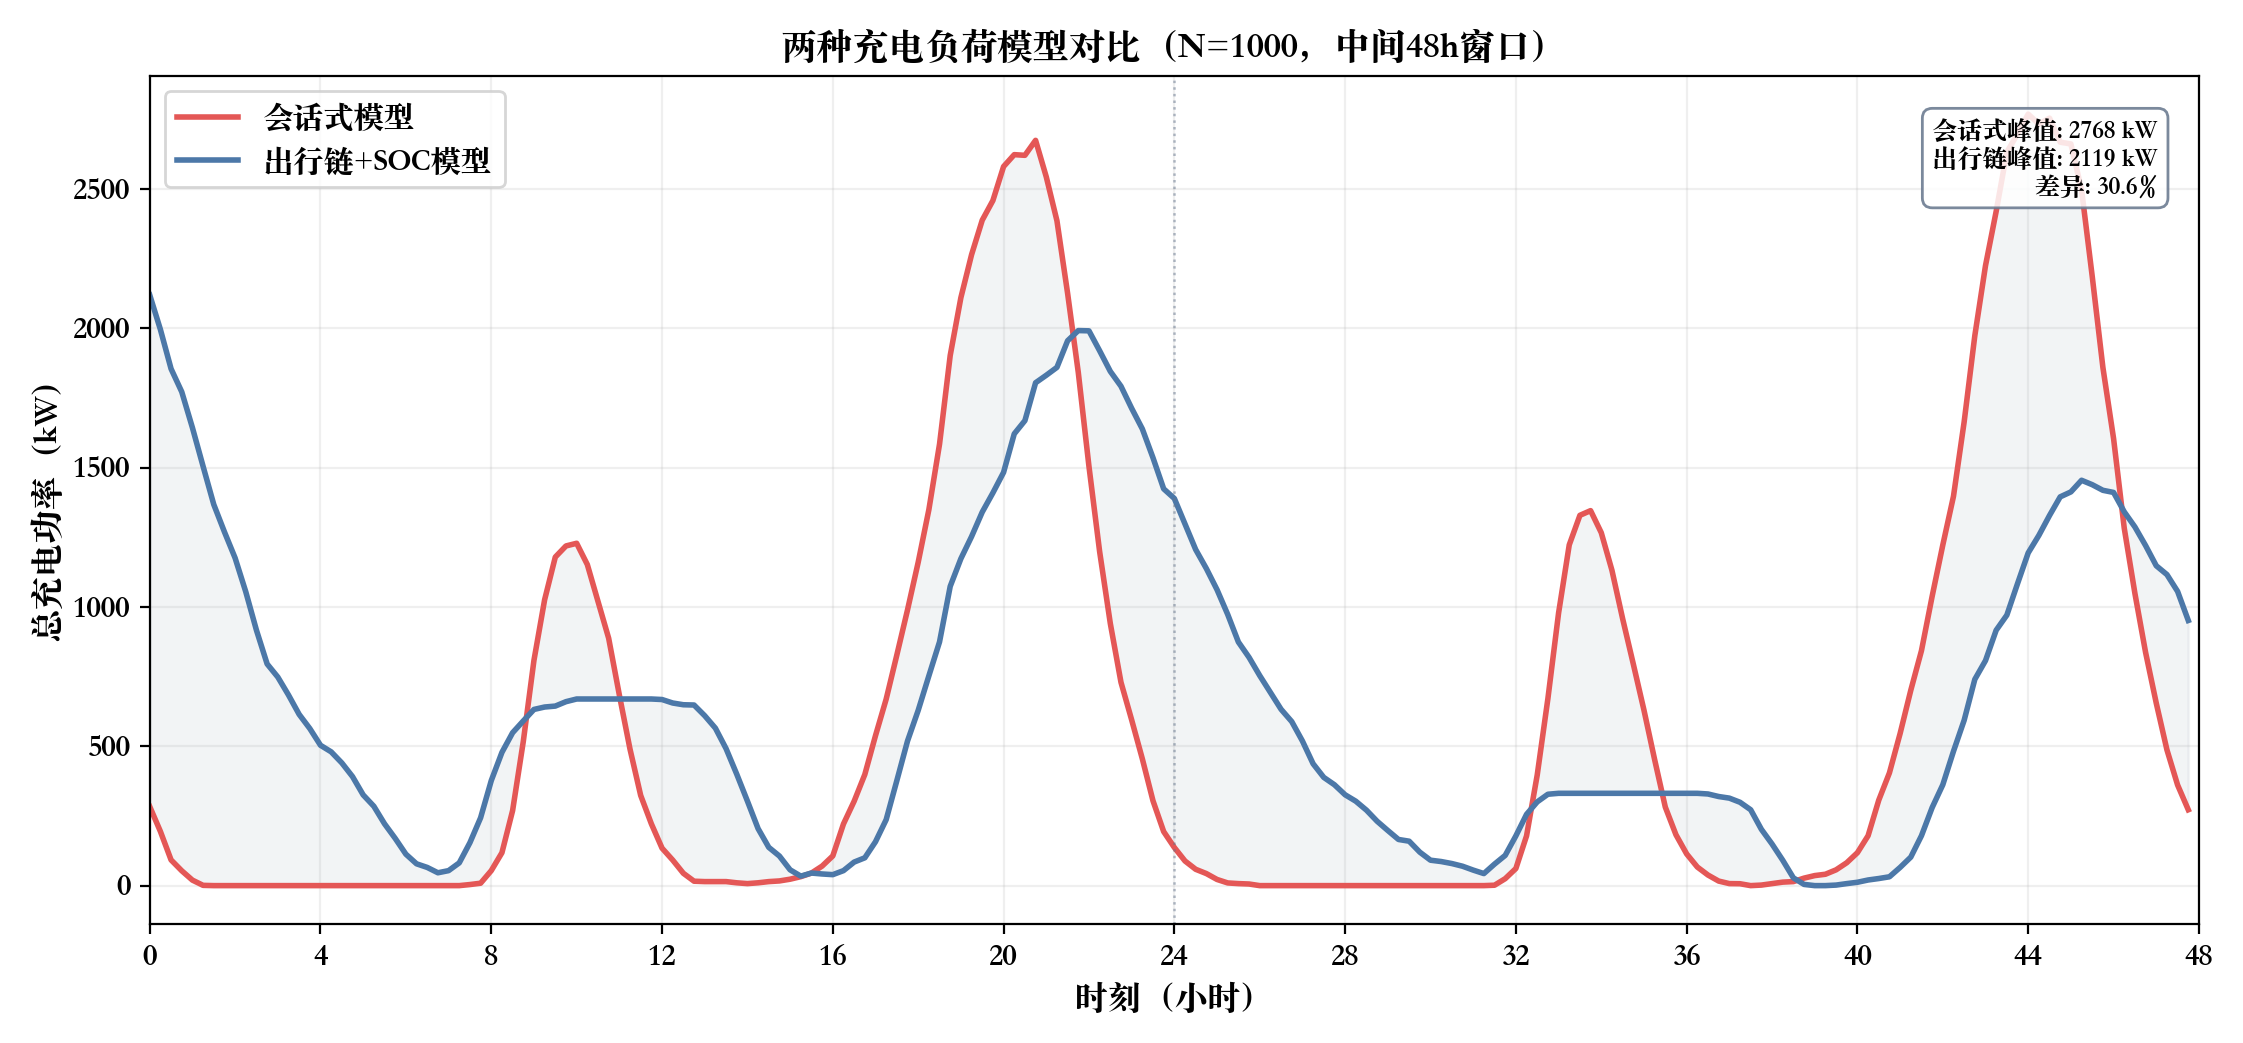
\includegraphics[width=0.86\textwidth]{fig_2_7.png}
        \caption{两种充电负荷模型对比（$N = 1000$，中间 48 h 窗口）}
        \label{fig:model_comparison}
    \end{figure}

    出行链模型与会话式模型生成的聚合充电负荷存在显著差异。为保证比较口径一致，图中同样展示扩展仿真截取的中间 48 h 窗口。出行链模型由于刻画了日内多次出行的时空分散性，部分车辆在工作地点或中间停靠点即触发充电，使得充电负荷在时间上更为分散，峰值功率相对较低；会话式模型的充电事件在时间上更为集中，峰值功率更高。从承载力评估的角度看，负荷的时间分散性有利于降低峰值功率对配电网的冲击，因此出行链模型下的承载力通常高于会话式模型，这一差异将在第 4 章中进行定量分析。

    \noindent\textbf{（3）日内出行-充电时空轨迹}

    \begin{figure}[htbp]
        \centering
        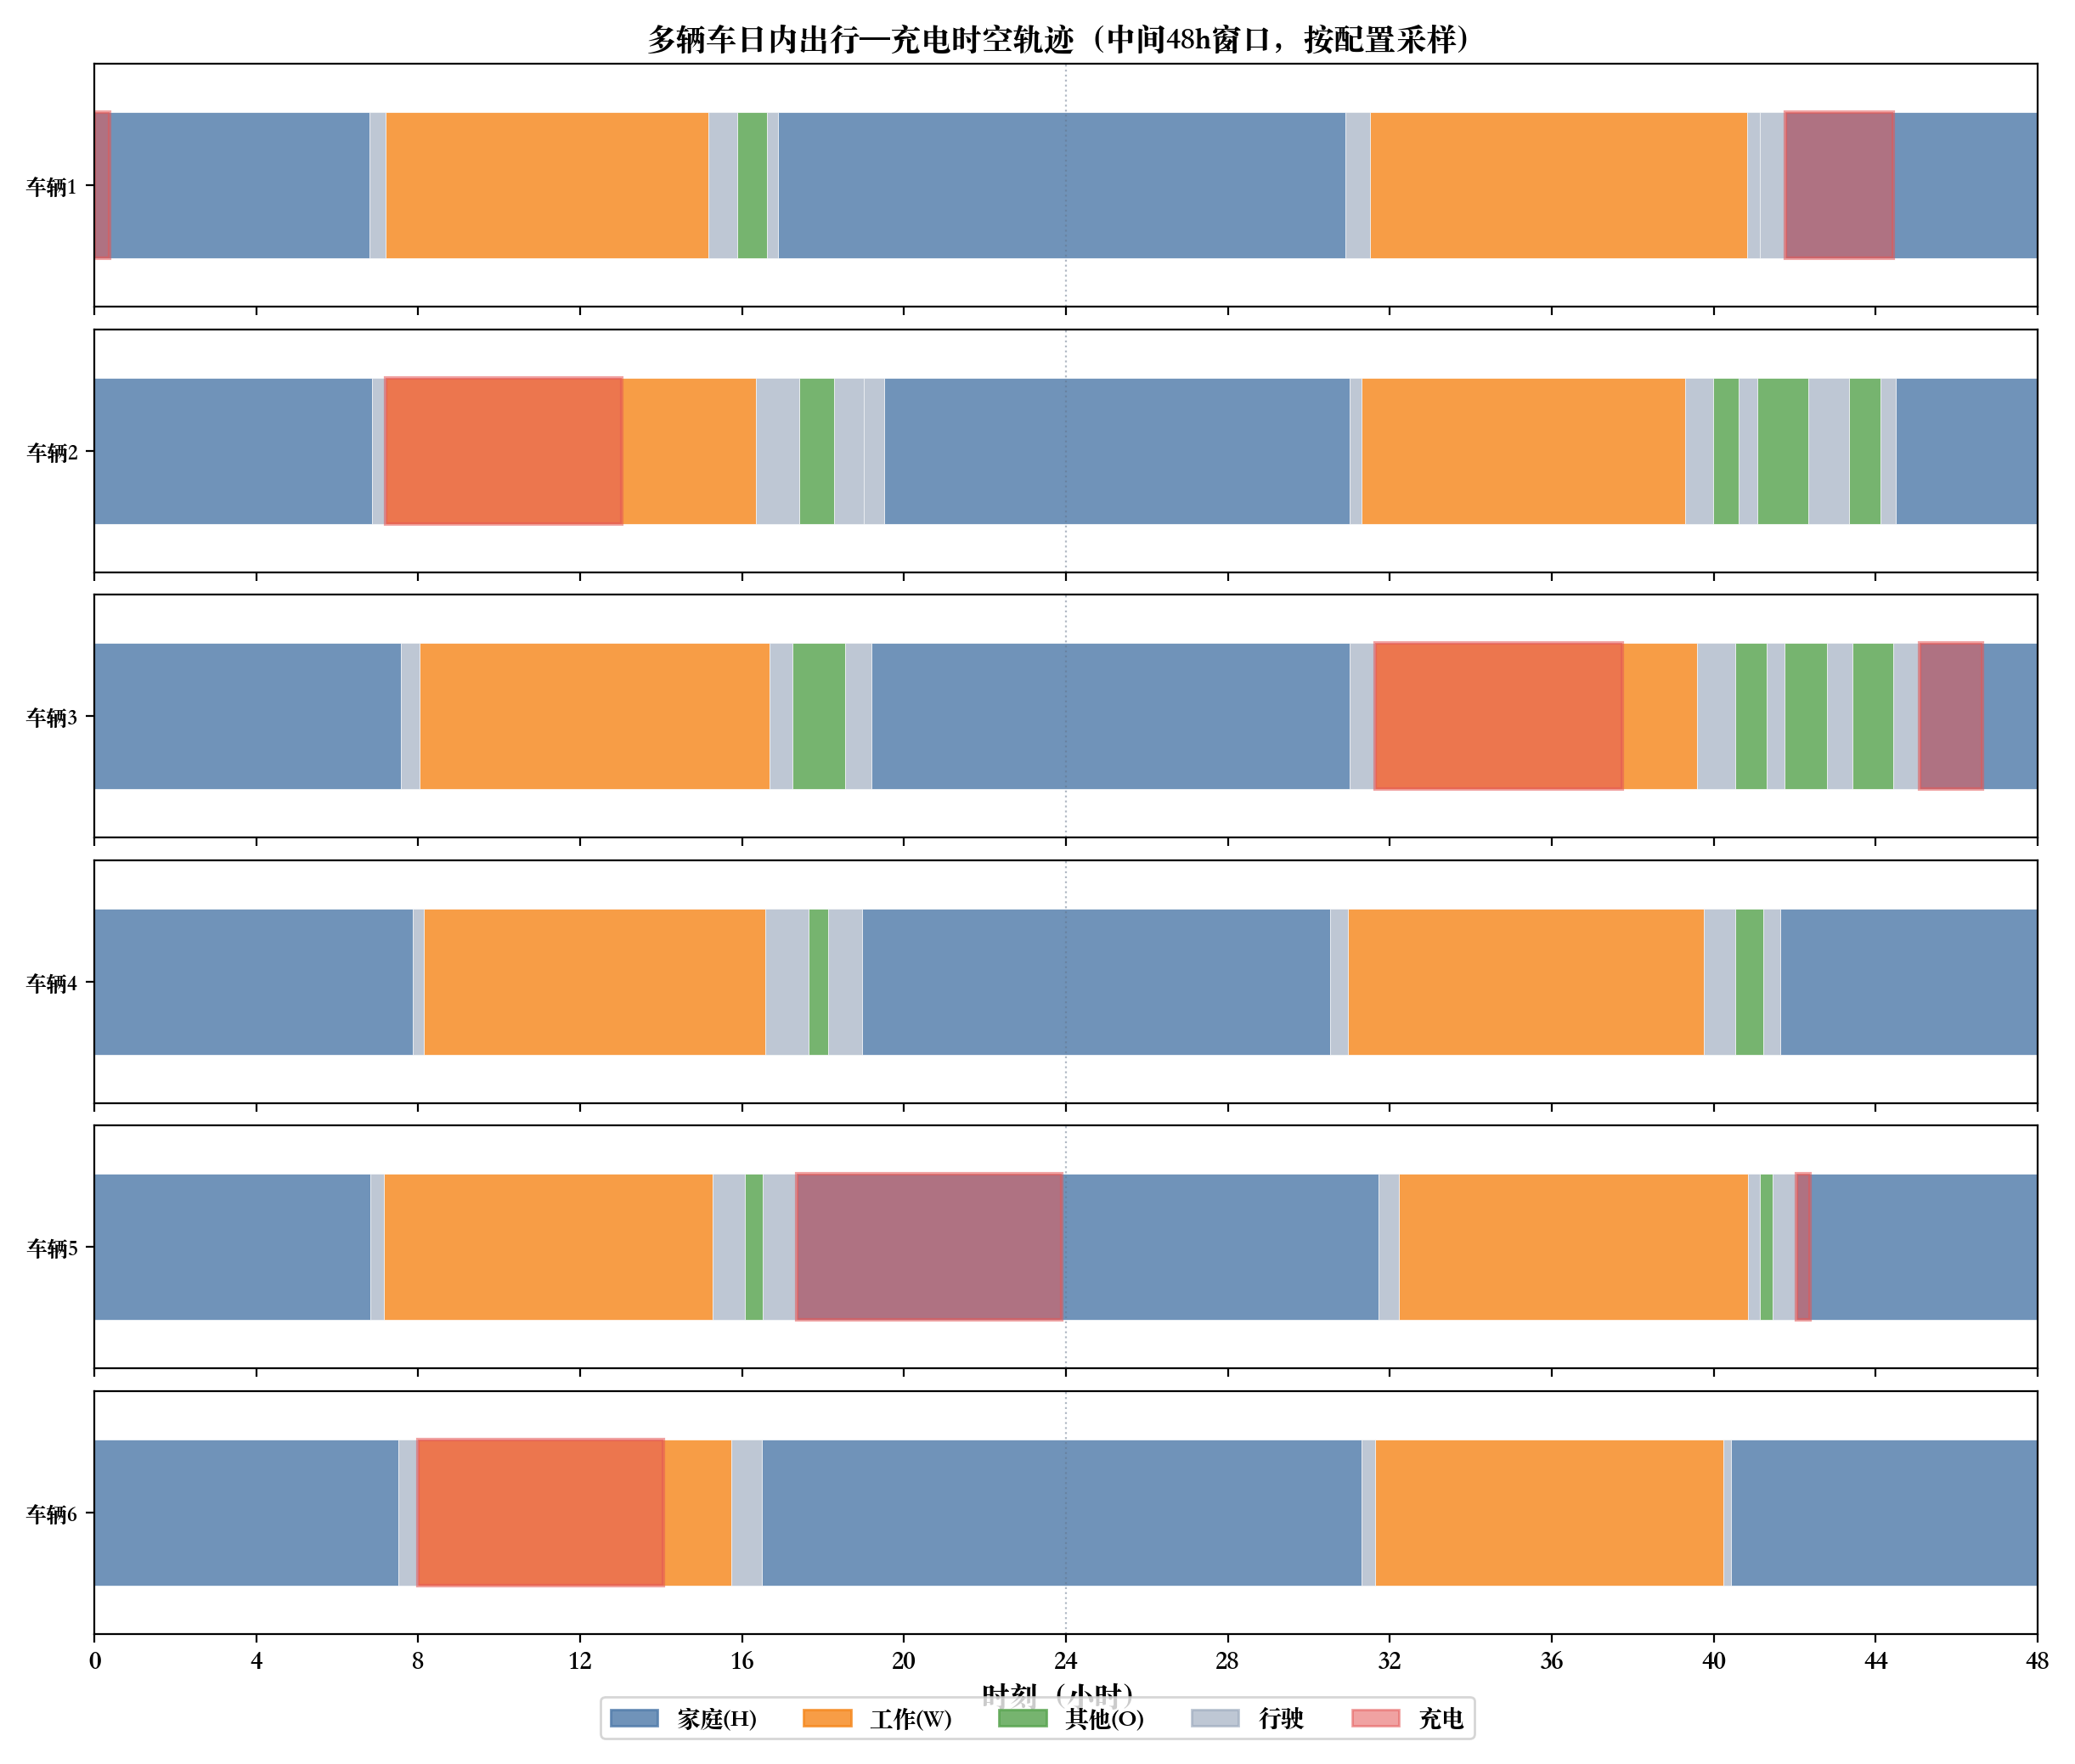
\includegraphics[width=0.82\textwidth]{fig_2_8.png}
        \caption{多辆车日内出行-充电时空轨迹（6 辆代表性车辆，中间 48 h 窗口）}
        \label{fig:travel_charging_trajectory}
    \end{figure}

    图 \ref{fig:travel_charging_trajectory} 与图 \ref{fig:aggregate_load_curve} 采用相同的配置参数和扩展仿真窗口，仅从候选车辆中选取覆盖“仅家庭充电”“仅工作地充电”“家庭与工作地均充电”以及“两日内无需充电”等不同模式的代表性样本。不同车辆的出发时间、工作时长、中间停靠次数和返家时间均存在随机差异，充电事件在时间和空间上的分布也因此呈现出丰富的多样性。这种行为层面的异质性是出行链模型捕捉充电负荷时空特征的根本优势。

    \noindent\textbf{（4）充电负荷母线级空间分布}

    \begin{figure}[htbp]
        \centering
        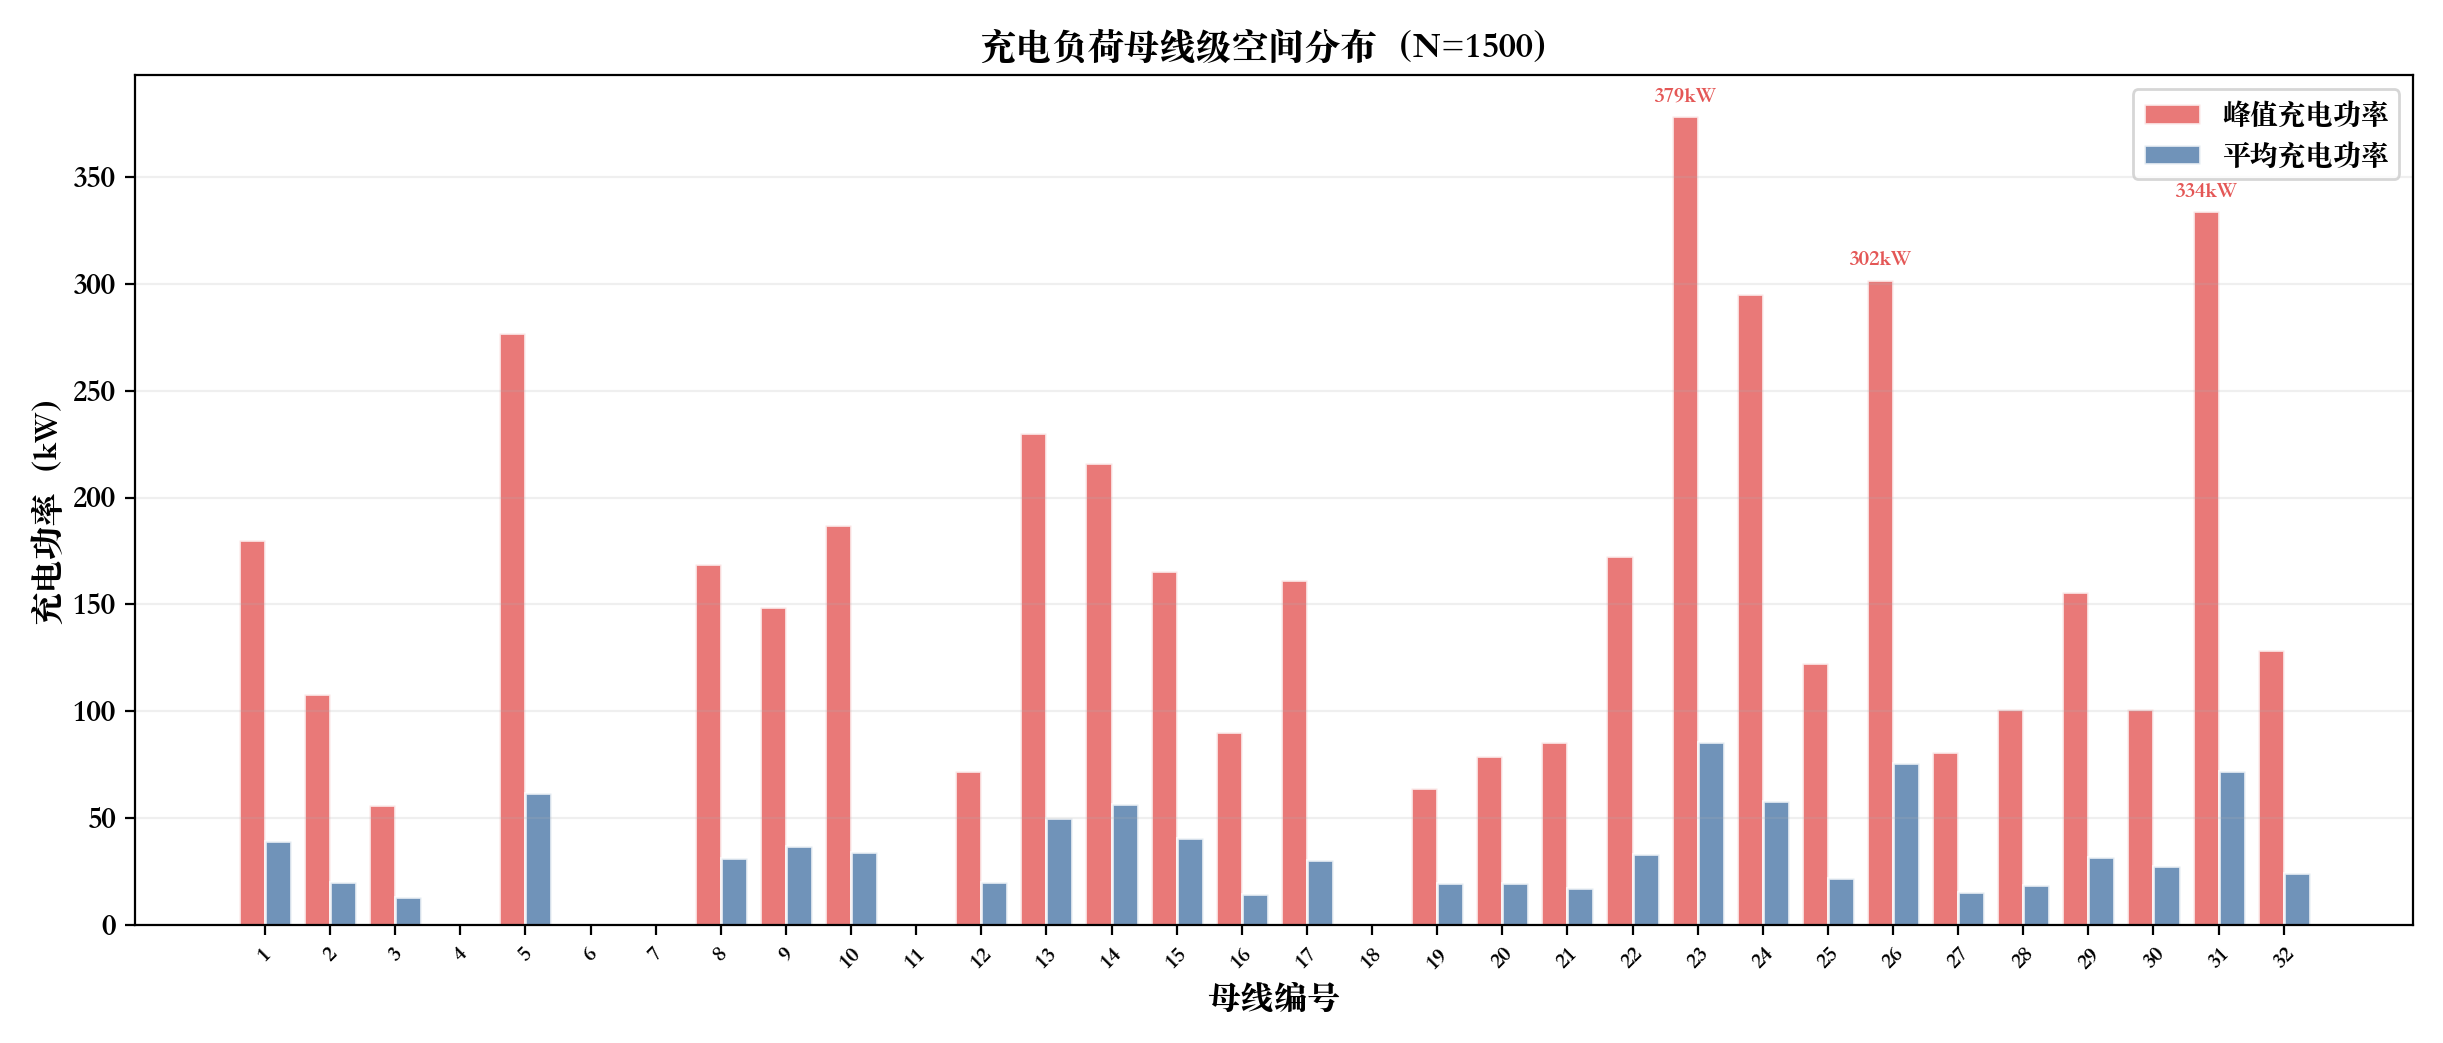
\includegraphics[width=0.86\textwidth]{fig_2_9.png}
        \caption{充电负荷母线级空间分布（$N = 1500$）}
        \label{fig:bus_level_load_distribution}
    \end{figure}

    充电负荷在配电网母线间的空间分布呈现显著的不均匀性。由于交通区域、母线映射的随机性以及不同区域出行活动强度的差异，各母线承担的充电功率存在较大差异。部分母线由于映射了多个高活动强度的交通区域而承担较大的充电负荷，而另一些母线的充电负荷较小。充电负荷的空间不均匀性直接影响配电网各节点的电压分布，是决定承载力瓶颈位置的关键因素。

    \subsection{本章小结}

    本章构建了基于出行链的电动汽车充电负荷时空建模方法，主要工作与结论如下：

    \noindent\textbf{（1）}
    建立了以“家 $\rightarrow$ 工作 $\rightarrow$ 中间停靠 $\rightarrow$ 家”为基本结构的出行链模型，各环节的首次出发时刻、行驶距离、工作驻留时长、中间停靠次数和停靠驻留时长等参数均通过校准的概率分布独立采样，完整刻画了日内多次出行的时空序列特征。

    \noindent\textbf{（2）}
    设计了多日连续仿真框架，通过逐日独立采样、时间偏移拼接和跨午夜停留合并三个步骤，克服了单日仿真在午夜截断充电窗口的缺陷，使 SOC 状态与充电会话能够自然跨越日边界延续，为有序充电等需要跨午夜窗口的策略提供了完整的仿真支撑。

    \noindent\textbf{（3）}
    建立了 SOC 状态演化方程与双层充电触发判据。行驶耗电通过单位里程能耗线性模型计算，充电补能以恒功率模式进行。充电触发由“下一程能量储备”判据与“末次居家补充充电”规则共同决定：前者综合考虑当前储能与下一段行程的能量需求，后者通过时间依赖的参与概率函数刻画车主在傍晚至夜间返家后主动插枪充电的行为习惯，并设定差异化的充电目标 SOC（补充充电取 0.9 而非充满），使模型所生成的晚高峰充电负荷更贴近实际。

    \noindent\textbf{（4）}
    建立了交通、电力耦合映射机制，通过映射矩阵将交通区域的充电需求投射至配电网母线，构建了母线级时序充电负荷矩阵作为后续潮流计算的直接输入。

    \noindent\textbf{（5）}
    实现了会话式模型作为对比基线，并分析了两种模型的充电负荷特性差异。出行链模型因刻画日内多次出行的时空分散性，充电负荷在时间上更为分散、峰值功率更低，有利于提升配电网承载力。

    % 第 3 章及后续章节待继续迁移至本文件。

\end{document}
